\section{Pipeline workshop}
\label{chap:workshop1}
	
	This workshop took place in . Attendants were asked to download all the datasets and install the free software QuPath for Part 1. Meanwhile, Part 2 required installing Cube Converter and Chemistry Simplifier for Windows 11 OS.
	
	The workshop introduced offline standalone software to process very large images: (1) Cube converter, (2) Chemistry simplifier, and (3) phase interpreter. They can be combined into image analysis pipelines for semi-automated mineralogy. The pipelines can be customised by the user and work on their PC to allow advanced navigation, pixel classification (QuPath software), object identification and dimensionality reduction applied to a variety of rock types (igneous, metamorphic, and sedimentary). 
	
	Using an example of a pyroxenite (websterite) thin section, the workshop demonstrated how image analysis tools can help to transition from subjective user-driven classification to more objective interpretation of object classes and their mutual relationships.
	
	\section{Workshop exercises}\label{workshop-exercises}	
	
	\subsection{Part 1}\label{part-1}
	
	\subsubsection{\texorpdfstring{Exercise 1: Demonstration by instructor - opening a 250 GB image. }{Exercise 1: Demonstration by instructor - opening a 250 GB image. }}\label{exercise-1-demonstration-by-instructor---opening-a-250-gb-image.}
	
	A huge pyramidal OME TIFF image can be opened in less than 5 seconds. The image data was saved in an external drive and the instructor will open it in his screen simply for demonstration.
	
	This shows that image formats are fundamental for the workflow. An example image pyramid is shown below.
	
	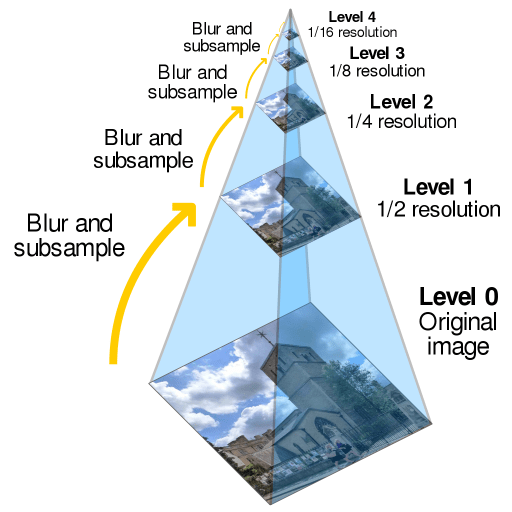
\includegraphics[width=2.33333in,height=2.33333in]{./media/image1.png}
	
	\subsubsection{Exercise 2: QuPath multi-view canvas}\label{exercise-2-qupath-multi-view-canvas}
	
	Please follow these steps on your PC:
	
	\begin{enumerate}
		\def\labelenumi{\arabic{enumi}.}
		\item
		Go to "../Seminar\_material/exercises\_data"
		\item
		Create an empty folder "../Seminar\_material/exercises\_data/exercise\_2"
		\item
		OPen QuPath and create a new project selecting that folder.
		\item
		In QuPath:
		
		\begin{enumerate}
			\def\labelenumii{\alph{enumii}.}
			\item
			Right-click in the black canvas \textgreater{} Multi-view \textgreater{} Synchronize viewers (deactivate)
			\item
			Right-click in the black canvas \textgreater{} Multi-view \textgreater{} Set grid size \textgreater{} Grid 2x2
			\item
			On the Project tab \textgreater{} Add images \textgreater{} Choose files \textgreater{}
			
			\begin{enumerate}
				\def\labelenumiii{\roman{enumiii}.}
				\item
				"..\textbackslash Seminar\_material\textbackslash exercises data\textbackslash registered\_pyramids\textbackslash montages\_original" \textgreater{} select all \textgreater{} Import
				\item
				"..\textbackslash Seminar\_material\textbackslash exercises data\textbackslash registered\_pyramids\textbackslash ama\_phasemap\_pyramid.tif"
				\item
				" ..\textbackslash Seminar\_material\textbackslash exercises data\textbackslash registered\_pyramids\textbackslash BSE\_pyramid.tif"
			\end{enumerate}
			\item
			All images should now be displayed in Data tree.
			\item
			Open the following four images:
			
			\begin{enumerate}
				\def\labelenumiii{\roman{enumiii}.}
				\item
				Click the first split (top left) \textgreater{} "ama\_phasemap\_pyramid.tif" (double click)
				\item
				Click the second split (top right) \textgreater{} "BSE\_pyramid.tif"
				\item
				Click the third split (top right) \textgreater{} "10x\_RL BF\_01\_z0.tif"
				\item
				Click the fourth split (bottom right) \textgreater{} "10x\_xpl-0\_01\_z0.tif"
			\end{enumerate}
			\item
			Right-click in the canvas \textgreater{} Multi-view \textgreater{} Synchronize viewers (activate).
			\item
			If the images are not perfectly aligned, click on ``Set the current viewer's zoom to fit the images'' (for each image) and re-synchronize\\
			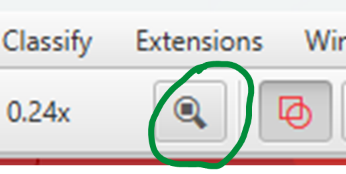
\includegraphics[width=1.57274in,height=0.79092in]{./media/image2.png}
		\end{enumerate}
	\end{enumerate}
	
	The successful canvas now looks like this. You can now seamlessly navigate between a phase map (top left), BSE (top right), reflected light (bottom left) and an XPL optical image (bottom right).
	
	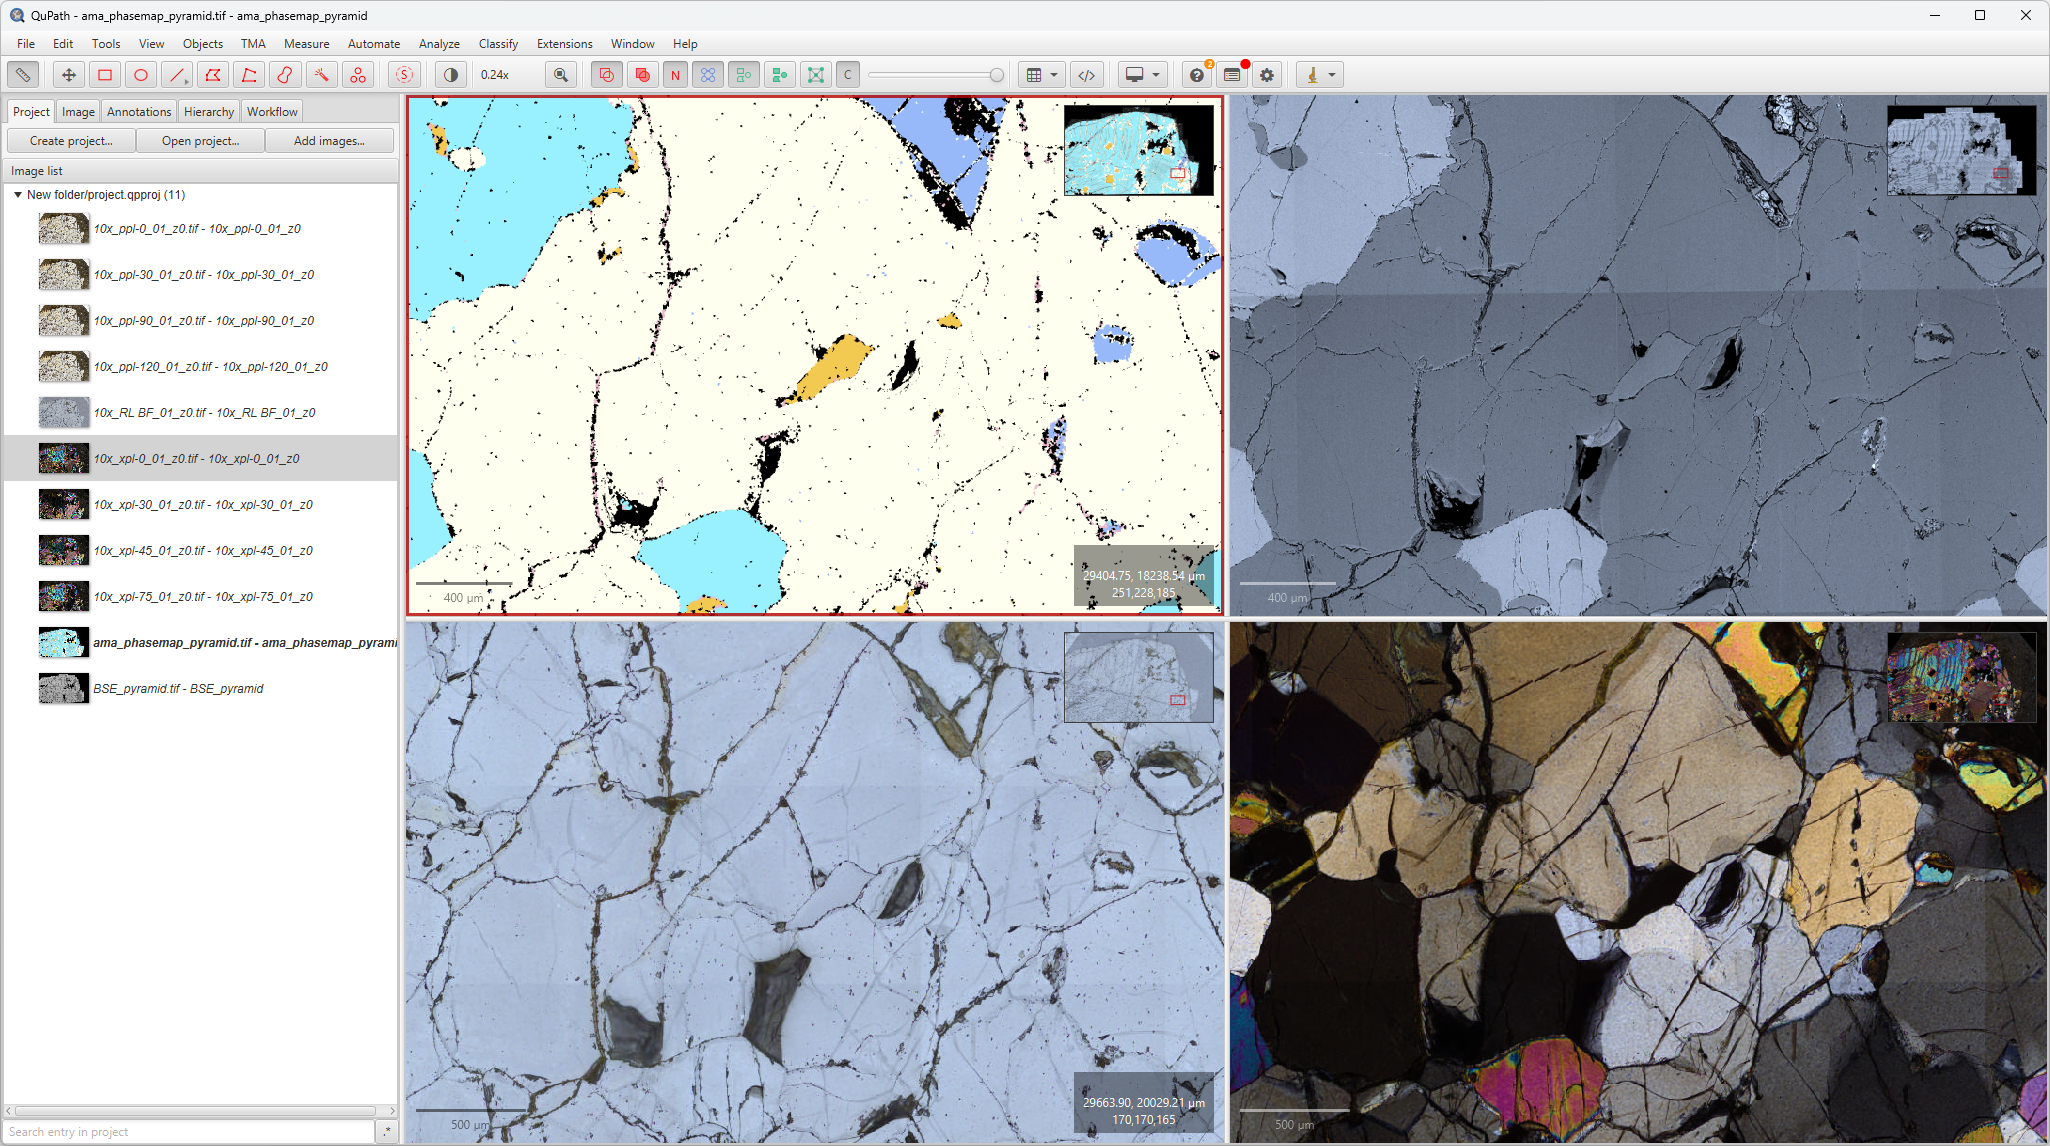
\includegraphics[width=6.26806in,height=3.50417in,alt={A screenshot of a computer screen AI-generated content may be incorrect.}]{./media/image3.png}
	
	\subsubsection{Exercise 3: `Boxing in' images within the multi-view canvas}\label{exercise-3-boxing-in-images-within-the-multi-view-canvas}
	
	You'll notice that there are many more images available in the data tree. While QuPath offers the option of using a 3x3 or larger canvas, simultaneously viewing such large numbers of images becomes counter-intuitive. To overcome this issue, we instead group related images into a single z-stack. For example, we can burn all optical images into a stack, or we can stack 6-12 chemical maps into a single stack. Each stack then only occupies one filed in the canvas and we instead flick between stack layers to display the various images within the stack. In the example below, you will generate a 2x2 canvas with all xpl images in a stack in the top left panel, all ppl images in a stack in the top right and one reflected light and one BSE image in the bottom two panels, respectively.
	
	On your PC follow these steps:
	
	\begin{enumerate}
		\def\labelenumi{\arabic{enumi}.}
		\item
		Go to "../Seminar\_material/exercises\_data"
		\item
		Create an empty folder "../Seminar\_material/exercises\_data/exercise\_3"
		\item
		Go to QuPath and create a new project selecting that folder.
		\item
		In QuPath:
		
		\begin{enumerate}
			\def\labelenumii{\alph{enumii}.}
			\item
			Right-click in the black canvas \textgreater{} Multi-view \textgreater{} Synchronize viewers (deactivate)
			\item
			Right-click in the black canvas \textgreater{} Multi-view \textgreater{} Set grid size \textgreater{} Grid 2x2
			\item
			On the Project tab \textgreater{} Add images \textgreater{} Choose files \textgreater{}
			
			\begin{enumerate}
				\def\labelenumiii{\roman{enumiii}.}
				\item
				"..\textbackslash Seminar\_material\textbackslash exercises data\textbackslash registered\_pyramids\textbackslash montages\_z-stack" \textgreater{} select all \textgreater{} Import
				\item
				"..\textbackslash Seminar\_material\textbackslash exercises data\textbackslash registered\_pyramids\textbackslash montages\_z-stack\textbackslash10x\_RL BF\_01\_z0.tif"
				\item
				"..\textbackslash Seminar\_material\textbackslash exercises data\textbackslash registered\_pyramids\textbackslash BSE\_pyramid.tif"
			\end{enumerate}
			\item
			All images should be displayed in Data tree.
			\item
			Open the following images:
			
			\begin{enumerate}
				\def\labelenumiii{\roman{enumiii}.}
				\item
				Click the first split (top left) \textgreater{} "xpl\_z-stack.tif" (double click)
				\item
				Click the second split (top right) \textgreater{} "ppl\_z-stack.tif"
				\item
				Click the third split (bottom left) \textgreater{} "10x\_RL BF\_01\_z0.tif"
				\item
				Click the fourth split (bottom right) \textgreater{} "BSE\_pyramid.tif"
			\end{enumerate}
			\item
			Right-click in the canvas \textgreater{} Multi-view \textgreater{} Synchronize viewers (activate).
			\item
			If the images are not perfectly aligned, click on ``Set the current viewer's zoom to fit the images'' (for each image) and re-synchronize\\
			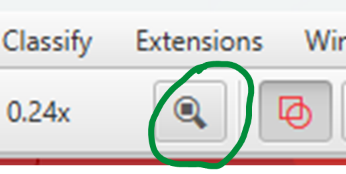
\includegraphics[width=1.57274in,height=0.79092in]{./media/image2.png}
		\end{enumerate}
	\end{enumerate}
	
	The successful canvas now looks like this:
	
	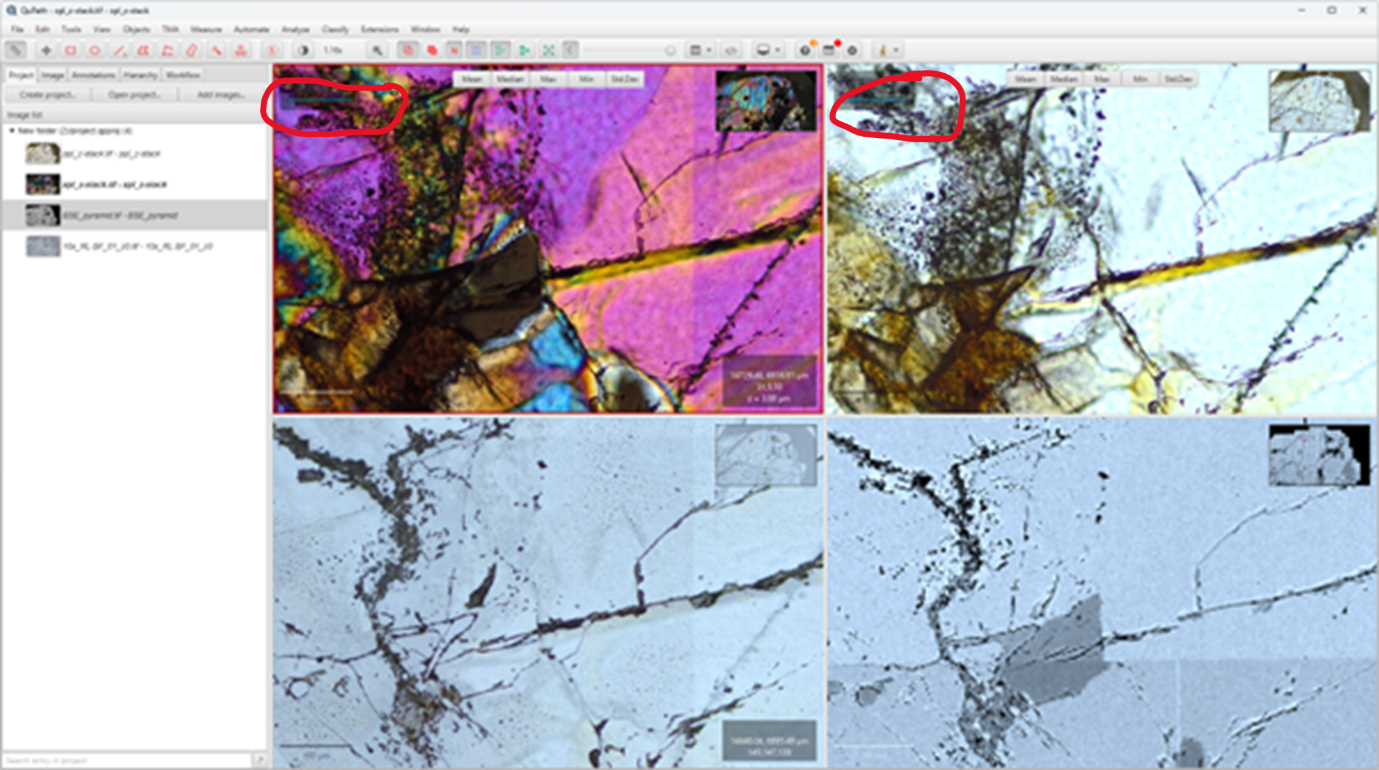
\includegraphics[width=6.26673in,height=3.50003in]{./media/image4.png}
	
	Note that the two z-stacks have a slider at the top left (in blue) that can be click-dragged to flick between images.
	
	\subsubsection{Exercise 4: Multi-view with ray tracing and dimensionality reduction}\label{exercise-4-multi-view-with-ray-tracing-and-dimensionality-reduction}
	
	In multimodal microscopy, with up to 20 imagery of the same specimen, our capacity to digest the incredible amount of information reaches its limits. Furthermore, for classifying pixels, the complexities of light interaction with anisotropic minerals confuse learning algorithms. To reduce these complexities, we have developed two methods which summarise the images:
	
	\begin{itemize}
		\item
		\href{https://www.mdpi.com/2075-163X/13/2/156}{Ray tracing}: performs descriptive statistics of the optical image stack as single images for each microscopy modality (PPL, XPL). The most useful image is the maximum RGB intensity, both in PPL and XPL. The latter is equivalent to a `circular polarisation' image.
		\item
		\href{https://doi.org/10.1016/j.chemgeo.2024.121997}{Chemical dimensionality reduction}: performs three different types of simplification of chemical image stacks via PCA, UMAP or DSA (see Part 2). In practice, PCA images, where RGB represent loadings on PC1, PC2 and PC3, do well at showing mineralogy (phase maps), while the neural network DSA can reveal faint zonations.
	\end{itemize}
	
	In the next exercise, you will generate a 2x2 canvas combining an optical stack, a BSE image, an SEM-EDX phase map and then a chemistry simplification stack.
	
	On your PC follow these steps:
	
	\begin{enumerate}
		\def\labelenumi{\arabic{enumi}.}
		\item
		Go to "../Seminar\_material/exercises\_data"
		\item
		Create an empty folder "../Seminar\_material/exercises\_data/exercise\_4"
		\item
		Go to QuPath and create a new project selecting that folder.
		\item
		In QuPath:
		
		\begin{enumerate}
			\def\labelenumii{\alph{enumii}.}
			\item
			Right-click in the black canvas \textgreater{} Multi-view \textgreater{} Synchronize viewers (deactivate)
			\item
			Right-click in the black canvas \textgreater{} Multi-view \textgreater{} Set grid size \textgreater{} Grid 2x2
			\item
			On the Project tab \textgreater{} Add images \textgreater{} Choose files \textgreater{}
			
			\begin{enumerate}
				\def\labelenumiii{\roman{enumiii}.}
				\item
				"..\textbackslash Seminar\_material\textbackslash exercises data\textbackslash registered\_pyramids\textbackslash montages\_z-stack\textbackslash optical-z-stack.tif" \textgreater{} Import
				\item
				"..\textbackslash Seminar\_material\textbackslash exercises data\textbackslash registered\_pyramids\textbackslash BSE\_pyramid.tif"
				\item
				"..\textbackslash Seminar\_material\textbackslash exercises data\textbackslash registered\_pyramids\textbackslash ama\_phasemap\_pyramid.tif"
				\item
				"..\textbackslash Seminar\_material\textbackslash exercises data\textbackslash registered\_pyramids\textbackslash montages\_z-stack\textbackslash reduced\_z-stack.tif"
			\end{enumerate}
			\item
			All images should be displayed in the Data tree.
			\item
			Open the following images:
			
			\begin{enumerate}
				\def\labelenumiii{\roman{enumiii}.}
				\item
				Click the first split (top left) \textgreater{} "optical\_z-stack.tif" (double click)
				\item
				Click the third split (top right) \textgreater{} "BSE\_pyramid.tif"
				\item
				Click the first split (bottom left) \textgreater{} "ama\_phasemap\_pyramid.tif"
				\item
				Click the fourth split (bottom right) \textgreater{} "reduced\_z-stack.tif "
			\end{enumerate}
			\item
			Right-click in the canvas \textgreater{} Multi-view \textgreater{} Synchronize viewers (activate).
			\item
			If the images are not perfectly aligned, click on ``Set the current viewer's zoom to fit the images'' (for each image) and re-synchronize\\
			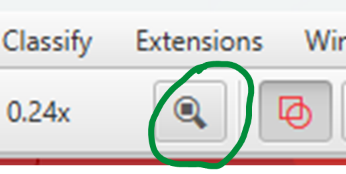
\includegraphics[width=1.57274in,height=0.79092in]{./media/image2.png}
		\end{enumerate}
	\end{enumerate}
	
	The successful output looks like this:
	
	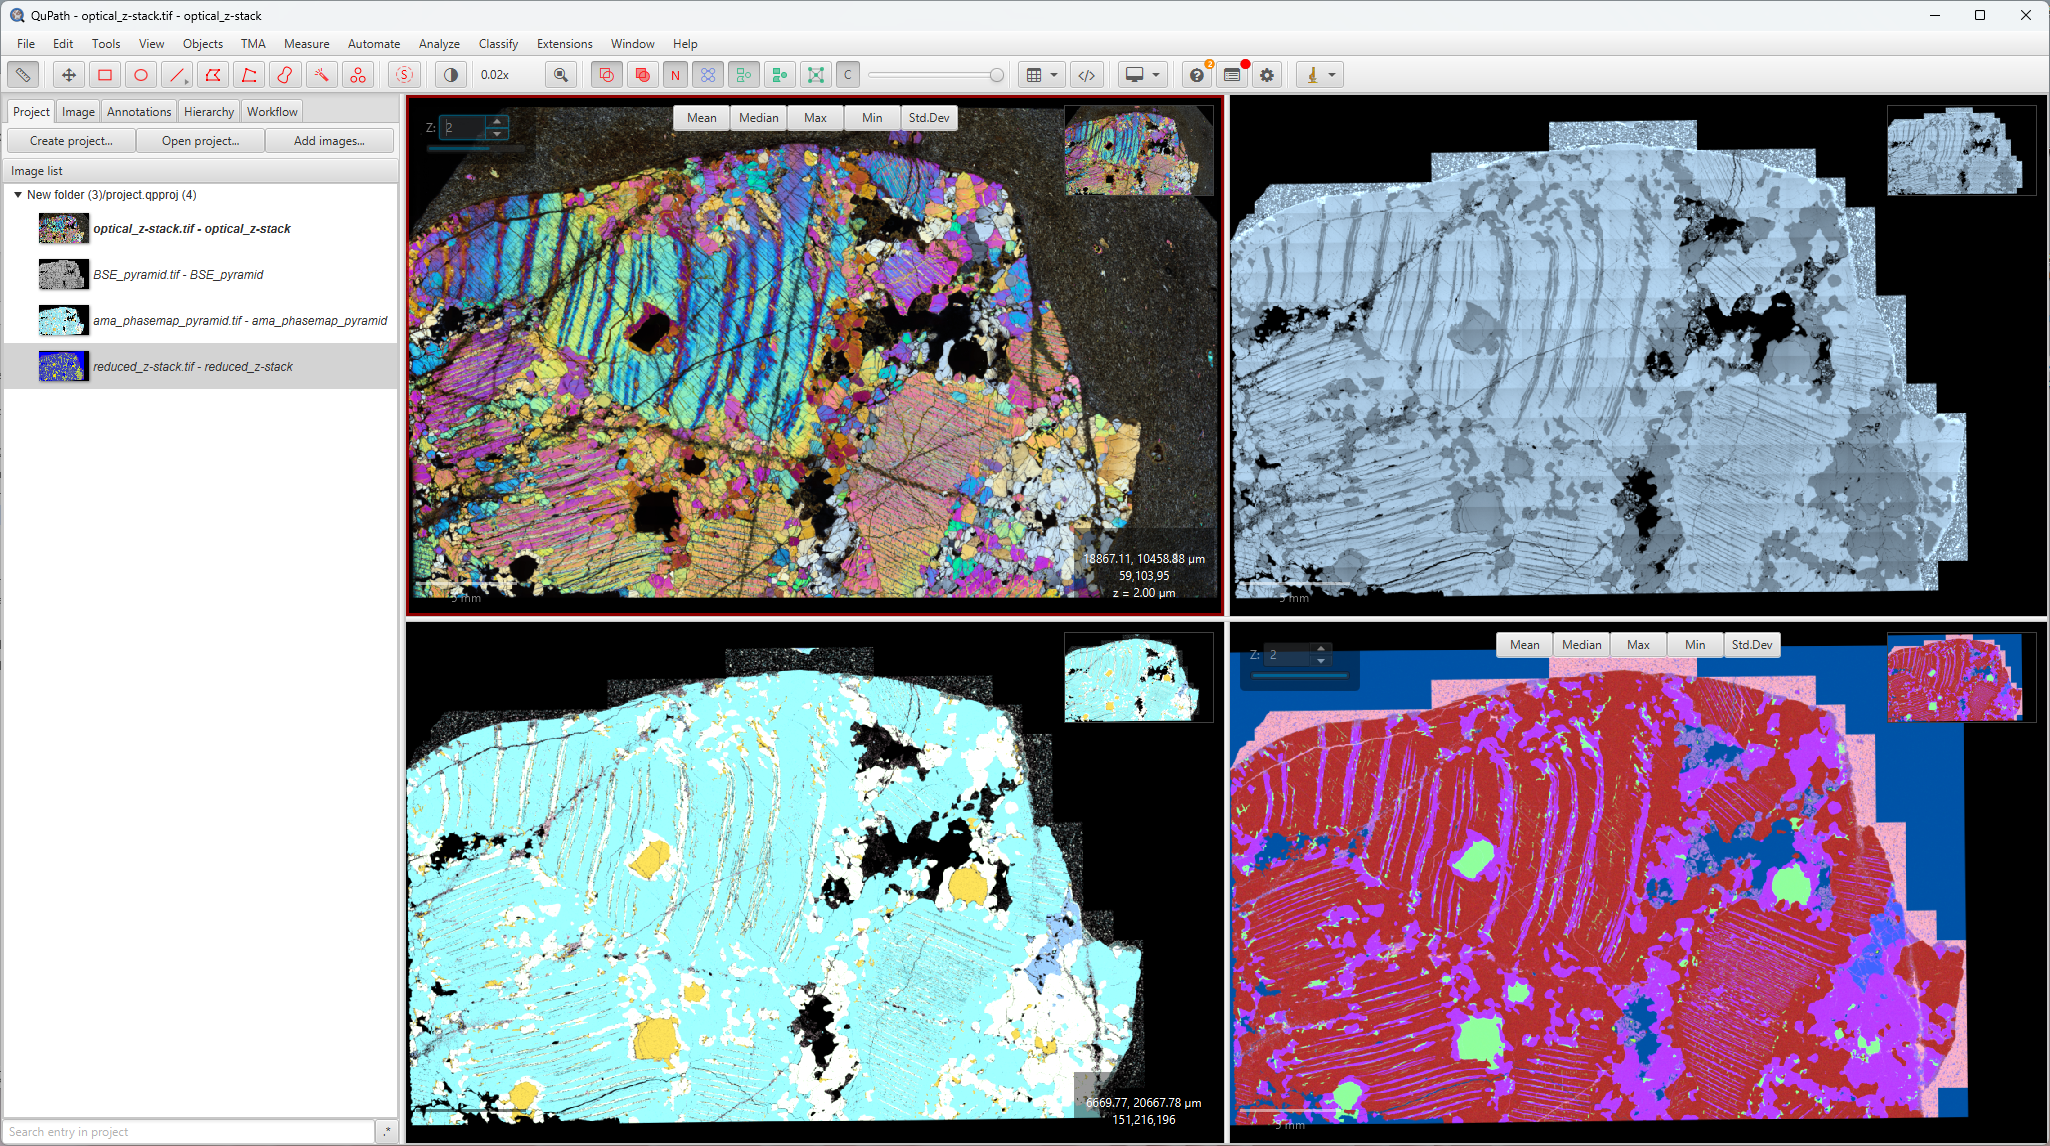
\includegraphics[width=6.26806in,height=3.50417in]{./media/image5.png}
	
	Not only are these images quicker to see but they can be studied with Machine/Deep learning algorithms. For example, QuPath allows drawing manual annotations (on each) and merging images and annotations into a multi-channel image (not a z-stack) for phase mapping using the ``Pixel Classifier'' (content of Part 2B).
	
	\subsection{Part 2A}\label{part-2a}
	
	This part is dedicated to Windows users.
	
	\subsubsection{Exercise 1: Ray tracing}\label{exercise-1-ray-tracing}
	
	When acquiring optical scans with slide scanners, a larger number of images are produced and saved in a ``data tree'' file. The QUT and UQ Evident VS200 slide scanners has been implemented to use polarisers and therefore serve as a petrographic microscope. In this exercise, you will use new software to crunch your stage rotation images (XPL-0, 15, 30, 45, ..) into summary representations. We call them XPL-(max, min, etc.) ray traced images.
	
	The outputs can be read in QuPath or in Evident ``software suite'' with ease and without paying for expensive software.
	
	On your PC follow these steps:
	
	\begin{enumerate}
		\def\labelenumi{\arabic{enumi}.}
		\item
		Open "../Seminar\_material/files/Cube Converter v1/Cube Converter v1.exe" (unzipped)
		\item
		(1) Polarised microscopy processor
		
		\begin{enumerate}
			\def\labelenumii{\alph{enumii}.}
			\item
			Image pyramid \textgreater{} Browse \textgreater{} "D:\textbackslash Seminar\_material\textbackslash exercises data\textbackslash optical\textbackslash Image\_03.vsi"
			\item
			Pyramid \textgreater{} level = 3
			\item
			Tiles and montages \textgreater{} All original scans
			\item
			Ray tracing options
			
			\begin{enumerate}
				\def\labelenumiii{\roman{enumiii}.}
				\item
				\textgreater{} PPL pleochroism and XPL birefringence (ticked on)
				\item
				\textgreater{} Maximum, Maximum index
			\end{enumerate}
			\item
			Run
		\end{enumerate}
	\end{enumerate}
	
	You were successful if the output looks like this:
	
	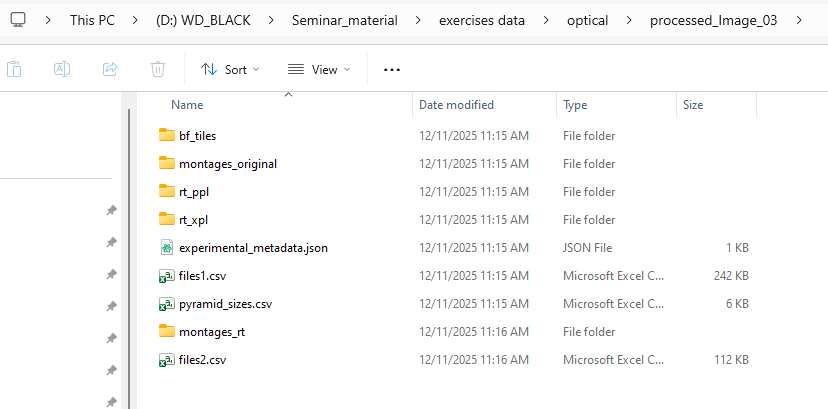
\includegraphics[width=6.26806in,height=3.09583in,alt={A screenshot of a computer AI-generated content may be incorrect.}]{./media/image6.png}
	
	The ``pyramid\_sizes.csv'' contains the experiment metadata for future reference:
	
	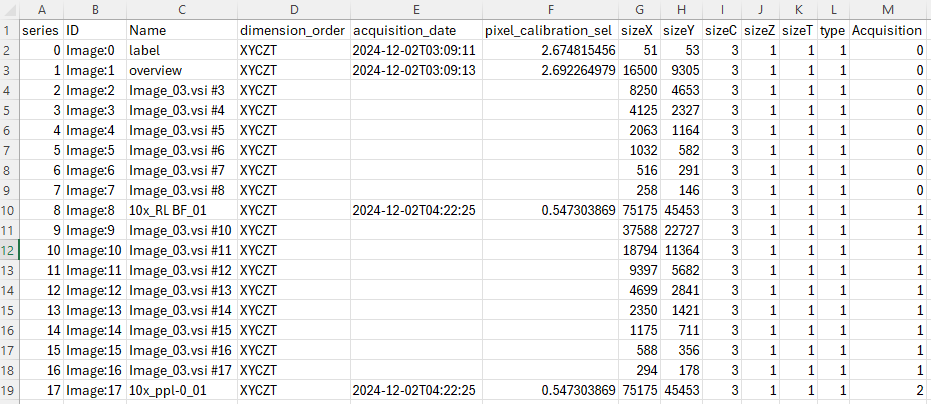
\includegraphics[width=5.99528in,height=2.6011in]{./media/image7.png}
	
	\subsubsection{Exercise 2: Making a z-stack}\label{exercise-2-making-a-z-stack}
	
	Z-stacks for biological samples are produced to vertically observe these tissue samples at different depths (the z-axis) for adjacent microtomed slices of the tissue. For us, mineral appearance (colour) changes in birefringent materials. In addition, the grains have random orientation/shape and relatively flat interiors that are not easily learnable.
	
	We developed the `hack' of using ``virtual'' z-stacks to see petrographic images in colour and different experiment orientations (not depths) while focusing at the sample surface (using reflected light). Balz calls them \ul{data cubes}. Cube converter (right hand side of interface) allows stacking optical and chemical images if they were pre-aligned (registered) with each other. I made a video detailing how to do align images with an ImageJ plugin, see ``booklet\_11-Nov-24\_extra materials.docx'' QUT routines (video \#2).
	
	On your PC follow these steps:
	
	\begin{enumerate}
		\def\labelenumi{\arabic{enumi}.}
		\item
		Open "../Seminar\_material/files/Cube Converter v1/Cube Converter v1.exe" (unzipped)
		\item
		(2) Multi-modal z-stack generator
		
		\begin{enumerate}
			\def\labelenumii{\alph{enumii}.}
			\item
			Input list:
			
			\begin{enumerate}
				\def\labelenumiii{\roman{enumiii}.}
				\item
				Add \textgreater{}
				
				\begin{enumerate}
					\def\labelenumiv{\arabic{enumiv}.}
					\item
					"..\textbackslash Seminar\_material\textbackslash exercises data\textbackslash registered\_pyramids\textbackslash montages\_original\textbackslash10x\_xpl-0\_01\_z0.tif"
					\item
					"..\textbackslash Seminar\_material\textbackslash exercises data\textbackslash registered\_pyramids\textbackslash montages\_original\textbackslash10x\_xpl-30\_01\_z0.tif"
					\item
					"..\textbackslash Seminar\_material\textbackslash exercises data\textbackslash registered\_pyramids\textbackslash montages\_original\textbackslash10x\_xpl-45\_01\_z0.tif"
					\item
					"..\textbackslash Seminar\_material\textbackslash exercises data\textbackslash registered\_pyramids\textbackslash montages\_original\textbackslash10x\_xpl-75\_01\_z0.tif"
				\end{enumerate}
			\end{enumerate}
			\item
			Pyramid calibration = 1.095 µm/pixel.
			
			\begin{enumerate}
				\def\labelenumiii{\roman{enumiii}.}
				\item
				If you do not know it. This can be calculated with:
			\end{enumerate}
		\end{enumerate}
	\end{enumerate}
	
	\[pixel\ size\ \left( \frac{µm}{px} \right) = \left( microscope\ objective\ calibration\left( \frac{µm}{px} \right) \right) \times \ 2^{pyramid\ level\ chosen}\]
	
	\begin{enumerate}
		\def\labelenumi{\alph{enumi}.}
		\setcounter{enumi}{2}
		\item
		Output file \textgreater{} my\_first\_z-stack
		\item
		Select Folder \textgreater{} create and choose a folder "..\textbackslash Seminar\_material\textbackslash exercises data\textbackslash registered\_pyramids\textbackslash montages\_z-stack" \textgreater{} Select Folder
		\item
		Run
	\end{enumerate}
	
	You were successful if the output looks like this:
	
	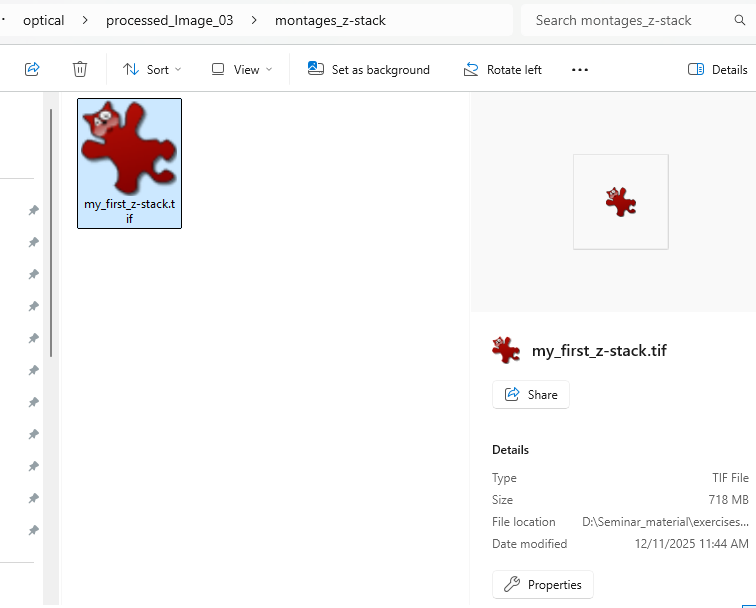
\includegraphics[width=3.5284in,height=2.83765in,alt={A screenshot of a computer AI-generated content may be incorrect.}]{./media/image8.png}
	
	\subsubsection{Exercise 3: Dimensionality reduction}\label{exercise-3-dimensionality-reduction}
	
	Chemistry simplifier software can be used to dimensionally reduce the number of chemical images into new red, green, and blue (RGB) images of high interpretability. In the guts of the software, randomly sampled pixels are used to factorise (Principal component ``PCA''), fit (Deep sparse autoencoder ``DSA''), and topologically approximate (Uniform manifold approximation and projection ``UMAP) a model that reduces the input chemical stack (SEM-EDX, XFM, XRF, spectra, etc.) into 3 channels. The model is then used to transform (parallel computation) the pixels of all the image while saving the process metadata required to reuse the models later (e.g., for scaling up to more thin sections).
	
	These ``representation'' images allow tracking element-mineral association without having to flick between too many images. In most commercial software, this is done using `composite' images for elemental combinations (e.g., Fe-K-Mg in a colourmap) that require a subjective choice of elements.
	
	On your PC follow these steps:
	
	\begin{enumerate}
		\def\labelenumi{\arabic{enumi}.}
		\item
		Open "../Seminar\_material/files/Chemistry Simplifier v1/Chemistry Simplifier v1.exe" (unzipped)
		\item
		(1) Pyramid generation and image processing
		
		\begin{enumerate}
			\def\labelenumii{\alph{enumii}.}
			\item
			Destination \textgreater{} "trial\_1"
			\item
			Experiments \textgreater{} "..\textbackslash Seminar\_material\textbackslash exercises data\textbackslash sem\textbackslash sem-edx\textbackslash after\_selected"
			\item
			Filtered search \textgreater{} (.+)
			\item
			Image format \textgreater{} png
		\end{enumerate}
		\item
		(2) Input and analysis definition
		
		\begin{enumerate}
			\def\labelenumii{\alph{enumii}.}
			\item
			Output\_tag \textgreater{} ``tag\_1''
			\item
			Click Refresh. Note that the list should auto-fill with the 16 images within the folder.
			\item
			Dimensionality reduction \textgreater{} Principal component analysis (ticked on)
		\end{enumerate}
		\item
		(3) Model parametrisation \textgreater{} Performance constraints \textgreater{} Downsampling \textgreater{} Scale = 1; Resolution = Full (1).
		
		\begin{enumerate}
			\def\labelenumii{\alph{enumii}.}
			\item
			\emph{If your computer is slow, please, use Scale = 2 and Resolution = 2}
		\end{enumerate}
		\item
		Run
	\end{enumerate}
	
	You were successful if the output looks like this:
	
	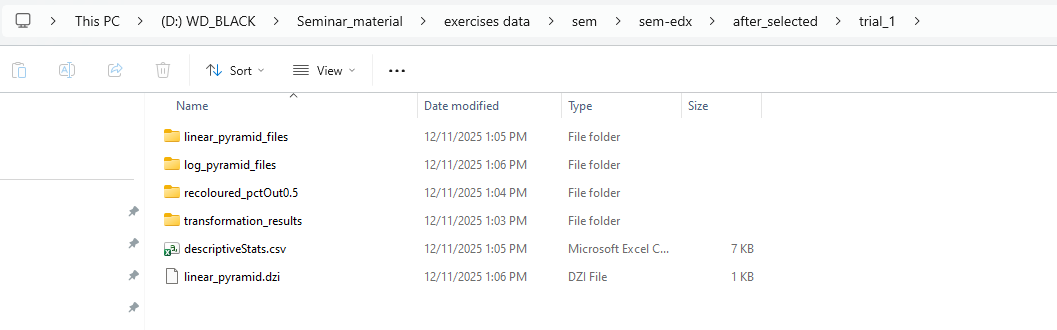
\includegraphics[width=6.26806in,height=1.95694in]{./media/image9.png}
	
	Containing a folder with recoloured images to help you know what images are not useful:
	
	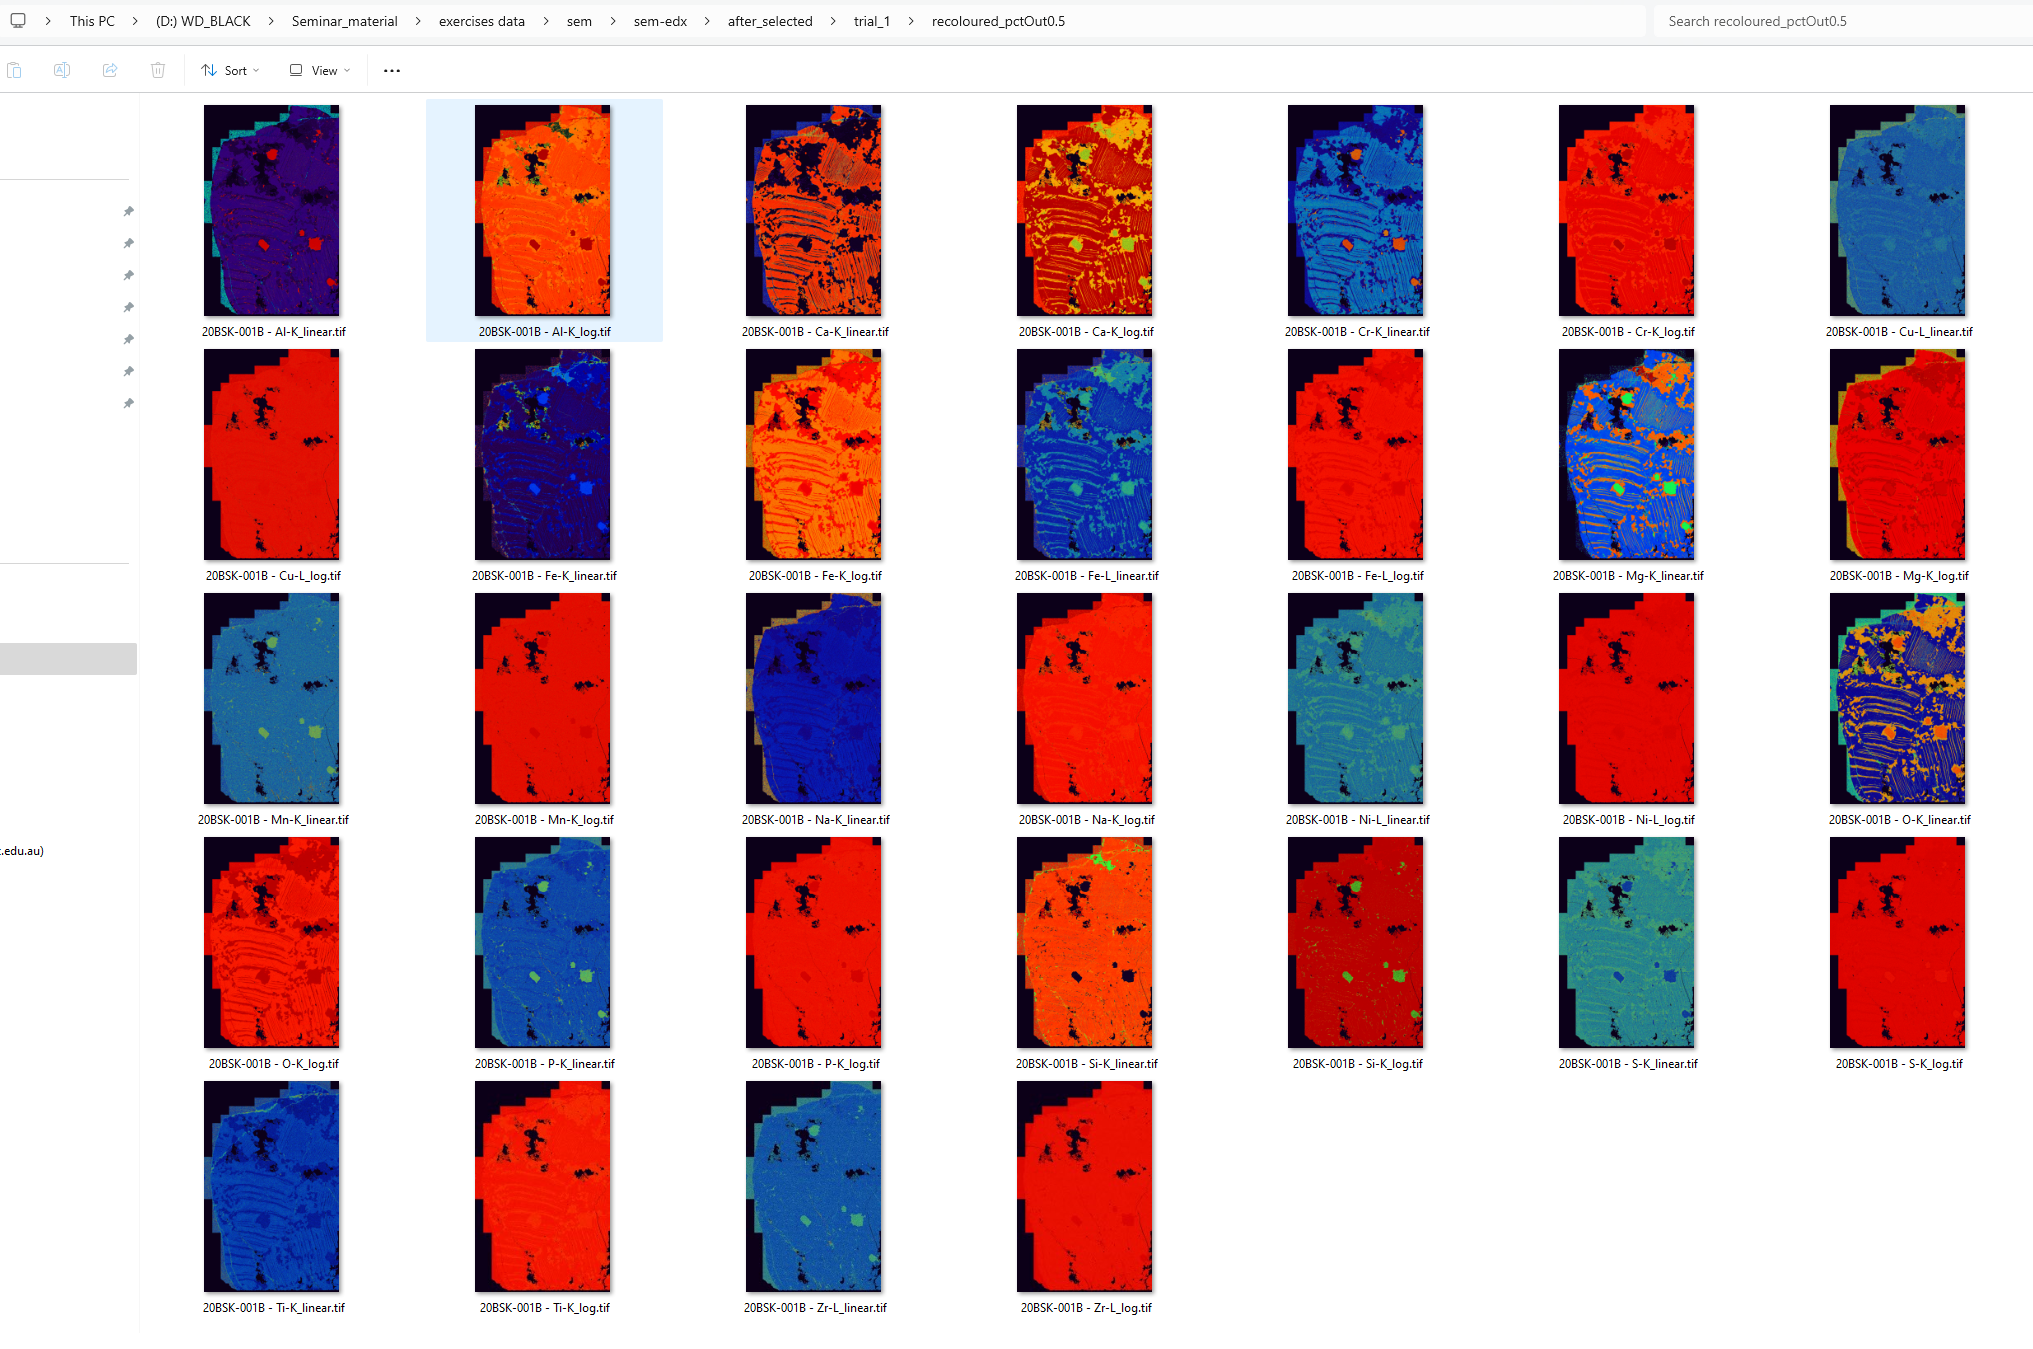
\includegraphics[width=6.26806in,height=4.15903in]{./media/image10.png}
	
	, and another folder containing the `tag' transformation output shown below. The ``montage\_pca.tif'' image has been opened (right-hand side) showing colour contrast between minerals:
	
	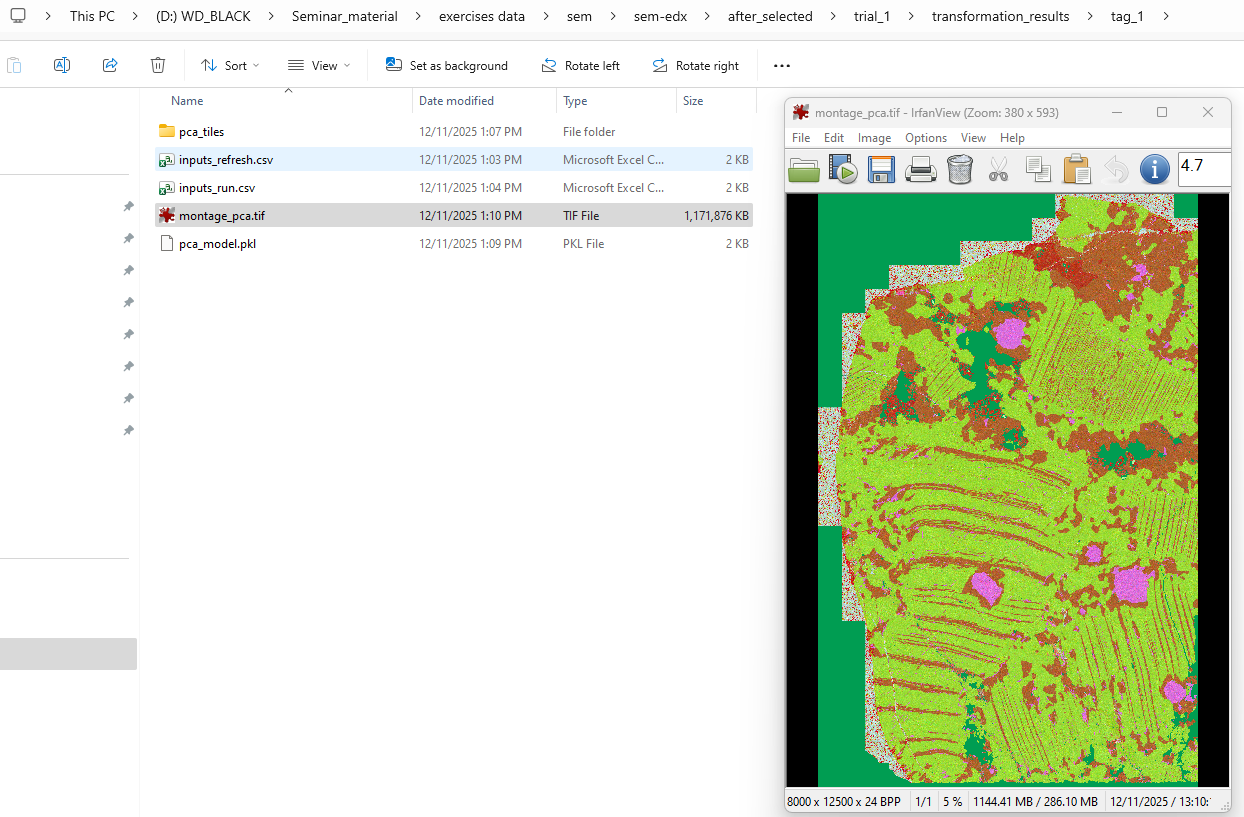
\includegraphics[width=6.14458in,height=4.03557in]{./media/image11.png}
	
	The DSA and UMAP transforms will not be used during this workshop, but you can try them at home (over night). If you are curious to view them, find them at:
	
	\begin{itemize}
		\item
		"D:\textbackslash Seminar\_material\textbackslash exercises data\textbackslash registered\_pyramids\textbackslash dsa\_selected\_artefacts\_8bit\_pyramid.tif"
		\item
		"D:\textbackslash Seminar\_material\textbackslash exercises data\textbackslash registered\_pyramids\textbackslash umap\_selected\_artefacts\_8bit\_pyramid.tif"
	\end{itemize}
	
	\subsection{Part 2B}\label{part-2b}
	
	This part is dedicated to Mac OS users.
	
	\subsubsection{Exercise 1: Phase mapping}\label{exercise-1-phase-mapping}
	
	QuPath was designed as a platform where users can see the deployment of image analysis algorithms with a tile-based system at multiple resolution scales (pyramids). The software includes pixel classification functionality that links images, annotations, and supervised learning models for semantic segmentation. In this exercise, you will learn to use the interface to annotate, train, and calibrate (in live mode) image segmentation in use of all the available dimensions within the input image stack.
	
	The key is to combine optical with dimensionally reduced chemical maps (read Part 2A), which ensures that the classifier has enough information to distingusih the `features' that we are interested in the sample and/or target minerals.
	
	We will ask you to use QuPath to:
	
	\begin{enumerate}
		\def\labelenumi{\Roman{enumi}.}
		\item
		Navigate the sample. Your petrographic microscopy knowledge will be key.
		\item
		Define annotation categories and draw polygon \ul{annotations} using the multi-view (see Part 1).
		\item
		Generate a `\ul{multi-channel} overlay'
		\item
		Transfer annotations to the overlay.
		\item
		Train a Random Tree model and save the model. Then, predict the map corresponding to that classifier within the QuPath project folder.
	\end{enumerate}
	
	Some level of familiarity with the Pixel classifier menu is required but we will mostly use default values today (try it at home).
	
	\paragraph{I. Navigation}\label{i.-navigation}
	
	On your PC, follow these steps:
	
	\begin{enumerate}
		\def\labelenumi{\arabic{enumi}.}
		\item
		Go to "../Seminar\_material/exercises\_data"
		\item
		Create an empty folder "../Seminar\_material/exercises\_data/exercise\_1"
		\item
		Go to QuPath and create a new project selecting that folder.
		\item
		In QuPath:
		
		\begin{enumerate}
			\def\labelenumii{\alph{enumii}.}
			\item
			Right-click in the black canvas \textgreater{} Multi-view \textgreater{} Synchronize viewers (deactivate)
			\item
			Right-click in the black canvas \textgreater{} Multi-view \textgreater{} Set grid size \textgreater{} Grid 2x2
			\item
			On the Project tab \textgreater{} Add images \textgreater{} Choose files \textgreater{}
			
			\begin{enumerate}
				\def\labelenumiii{\roman{enumiii}.}
				\item
				"..\textbackslash Seminar\_material\textbackslash exercises data\textbackslash registered\_pyramids\textbackslash montages\_rt\textbackslash xpl\_max\_z0.tif" \textgreater{} Import
				\item
				"..\textbackslash Seminar\_material\textbackslash exercises data\textbackslash registered\_pyramids\textbackslash montages\_original\textbackslash10x\_RL BF\_01\_z0.tif"
				\item
				"..\textbackslash Seminar\_material\textbackslash exercises data\textbackslash registered\_pyramids\textbackslash BSE\_pyramid.tif"
				\item
				".. \textbackslash Seminar\_material\textbackslash exercises data\textbackslash registered\_pyramids\textbackslash pca\_selected\_artefacts\_8bit\_pyramid.tif"
			\end{enumerate}
			\item
			All images should be displayed in the Data tree.
			\item
			Open the following images:
			
			\begin{enumerate}
				\def\labelenumiii{\roman{enumiii}.}
				\item
				Click the first split (top left) \textgreater{} "xpl\_max\_z0.tif" (double click)
				\item
				Click the third split (top right) \textgreater{} "10x\_RL BF\_01\_z0.tif"
				\item
				Click the first split (bottom left) \textgreater{} "BSE\_pyramid.tif"
				\item
				Click the fourth split (bottom right) \textgreater{} "pca\_selected\_artefacts\_8bit\_pyramid.tif"
			\end{enumerate}
			\item
			Right-click in the canvas \textgreater{} Multi-view \textgreater{} Synchronize viewers (activate).
			\item
			If the images are not perfectly aligned, click on ``Set the current viewer's zoom to fit the images'' (for each image) and re-synchronize\\
			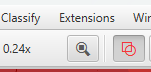
\includegraphics[width=1.57314in,height=0.7501in,alt={A screenshot of a computer AI-generated content may be incorrect.}]{./media/image12.png}
		\end{enumerate}
	\end{enumerate}
	
	You were successful if you output looks like this:
	
	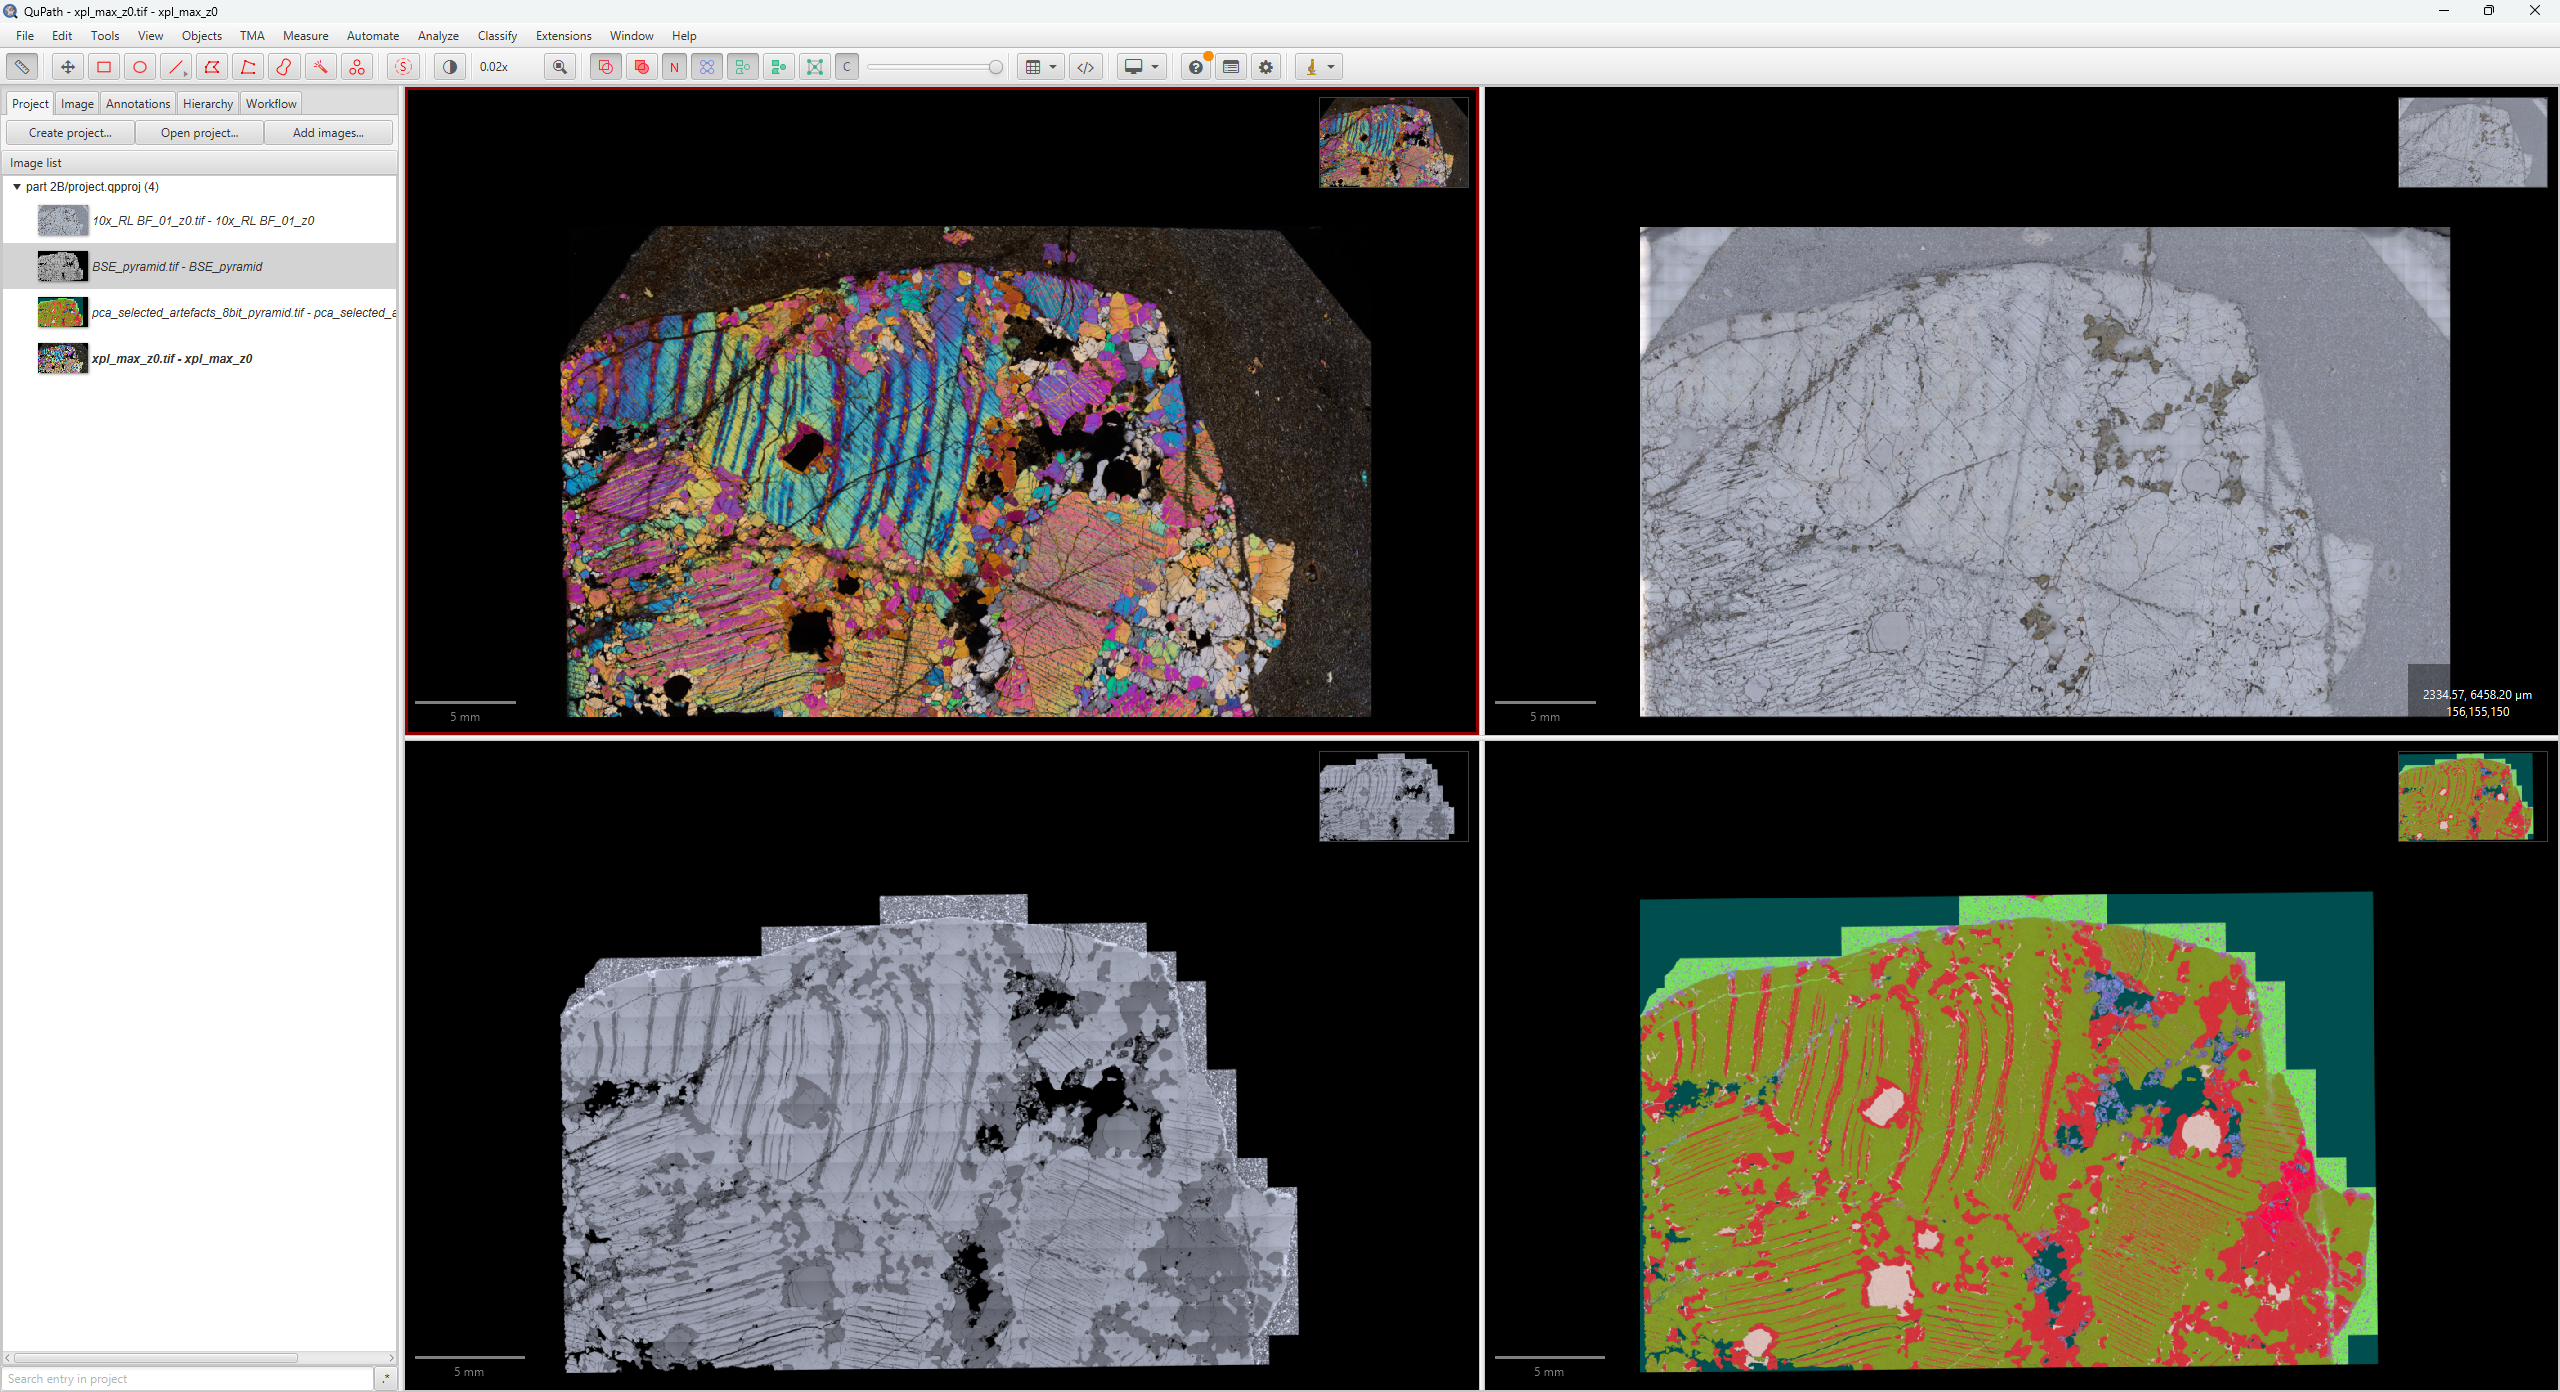
\includegraphics[width=6.26806in,height=3.40833in]{./media/image13.png}
	
	\paragraph{II. Annotation}\label{ii.-annotation}
	
	In your QuPath project, follow these steps:
	
	\begin{enumerate}
		\def\labelenumi{\arabic{enumi}.}
		\item
		Go to the Annotations tab
		\item
		Add items to the class list:
		
		\begin{enumerate}
			\def\labelenumii{\alph{enumii}.}
			\item
			click the ``+'' button (in red below)
			\item
			cpx, opx, grt, spn, olv, background, hole
		\end{enumerate}
		\item
		Change the colour of each category: click square next to each class (in blue below) and select a new colour. Follow the legend at last page of the \ul{booklet} printout.
	\end{enumerate}
	
	{\def\LTcaptype{none} % do not increment counter
		\begin{longtable}[]{@{}
				>{\raggedright\arraybackslash}p{(\linewidth - 2\tabcolsep) * \real{0.2939}}
				>{\raggedright\arraybackslash}p{(\linewidth - 2\tabcolsep) * \real{0.3160}}@{}}
			\toprule\noalign{}
			\begin{minipage}[b]{\linewidth}\raggedright
				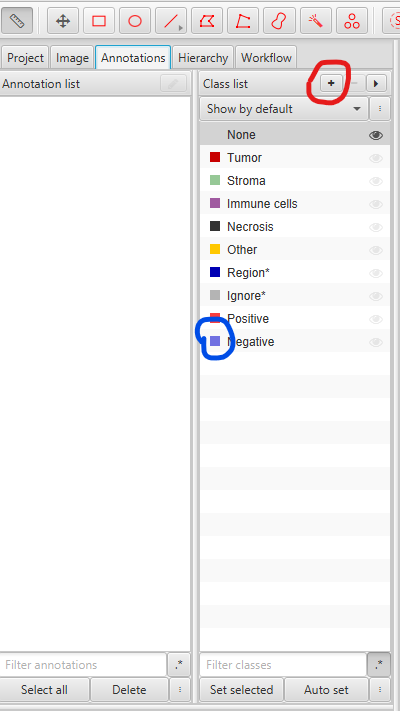
\includegraphics[width=1.68187in,height=2.98952in]{./media/image14.png}
			\end{minipage} & \begin{minipage}[b]{\linewidth}\raggedright
				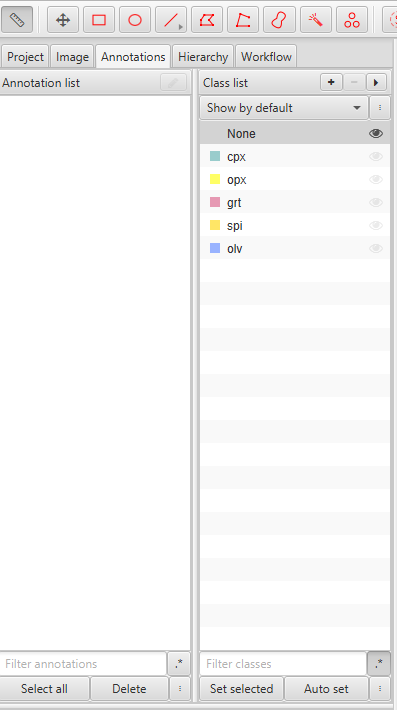
\includegraphics[width=1.67169in,height=2.98967in]{./media/image15.png}
			\end{minipage} \\
			\midrule\noalign{}
			\endhead
			\bottomrule\noalign{}
			\endlastfoot
		\end{longtable}
	}
	
	\begin{enumerate}
		\def\labelenumi{\arabic{enumi}.}
		\setcounter{enumi}{3}
		\item
		Annotate each class.
		
		\begin{enumerate}
			\def\labelenumii{\alph{enumii}.}
			\item
			In the canvas, choose an image where you feel you can do a good annotation.
			\item
			Draw polygons on top of each mineral class. The `brush' and `wand' tools are useful.
		\end{enumerate}
	\end{enumerate}
	
	
\includegraphics[width=4.45896in,height=0.46882in]{./media/image16.png}
	
	\begin{enumerate}
		\def\labelenumi{\alph{enumi}.}
		\setcounter{enumi}{2}
		\item
		In the example below: right-click the annotation (yellow contour) \textgreater{} Set classification \textgreater{} ``cpx''
	\end{enumerate}
	
	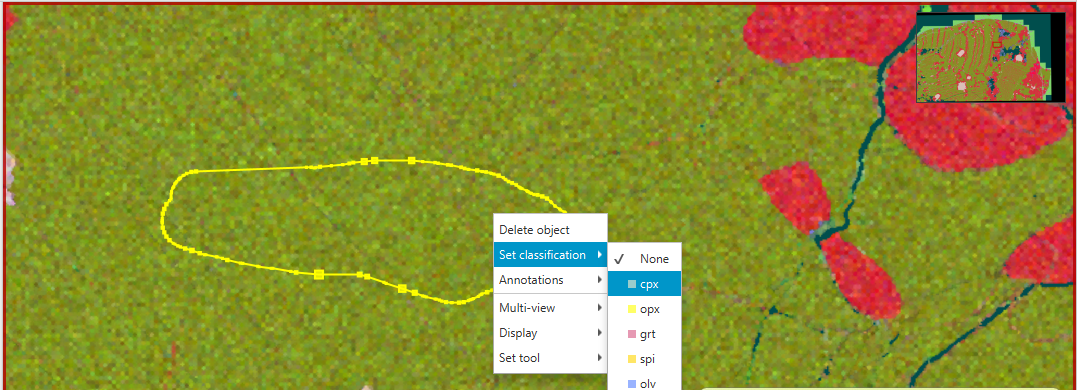
\includegraphics[width=5.26037in,height=1.9046in]{./media/image17.png}
	
	\begin{enumerate}
		\def\labelenumi{\alph{enumi}.}
		\setcounter{enumi}{3}
		\item
		The process is satisfactory usually when you have 3 or 4 annotations per class.
	\end{enumerate}
	
	\begin{enumerate}
		\def\labelenumi{\arabic{enumi}.}
		\setcounter{enumi}{4}
		\item
		When completed, go to Menu toolbar \textgreater{} File \textgreater{} Save.
		\item
		Repeat for each image if you \ul{annotated multiple images} in the canvas*.
	\end{enumerate}
	
	*The annotations are saved within each image. If switching images (or the project) you need to save your progress (File \textgreater{} Save).
	
	\paragraph{III. Generate multi-channel stack (overlay)}\label{iii.-generate-multi-channel-stack-overlay}
	
	First, we need to install a QuPath extension for image registration (only once):
	
	\begin{enumerate}
		\def\labelenumi{\arabic{enumi}.}
		\item
		Go to Menu toolbar \textgreater{} Extensions \textgreater{} Manage extensions \textgreater{} Manage extensions catalogs (button)
		\item
		Catalog URL (copy-paste: \url{https://github.com/BIOP/qupath-biop-catalog}) \textgreater{} Add
		\item
		Exit and reopen the software and open your project.
	\end{enumerate}
	
	In your reopened QuPath project, follow these steps:
	
	\begin{enumerate}
		\def\labelenumi{\arabic{enumi}.}
		\item
		Open an image in the canvas (double click in the data tree). For example, ``BSE\_pyramid.tif''.
		\item
		Go to Menu bar \textgreater{} Analyze \textgreater{} Interactive image combiner Warpy
	\end{enumerate}
	
	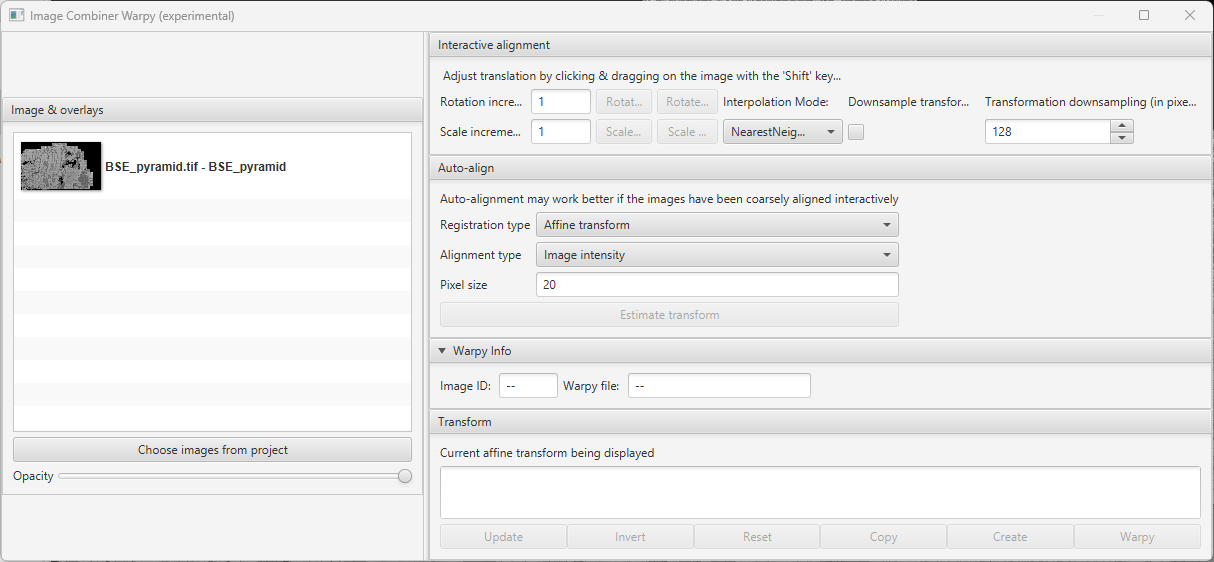
\includegraphics[width=5.78844in,height=2.67938in,alt={A screenshot of a computer AI-generated content may be incorrect.}]{./media/image18.png}
	
	\begin{enumerate}
		\def\labelenumi{\arabic{enumi}.}
		\setcounter{enumi}{2}
		\item
		Choose images from project \textgreater{} select all \textgreater{} OK
		\item
		Click \ul{Create}*
	\end{enumerate}
	
	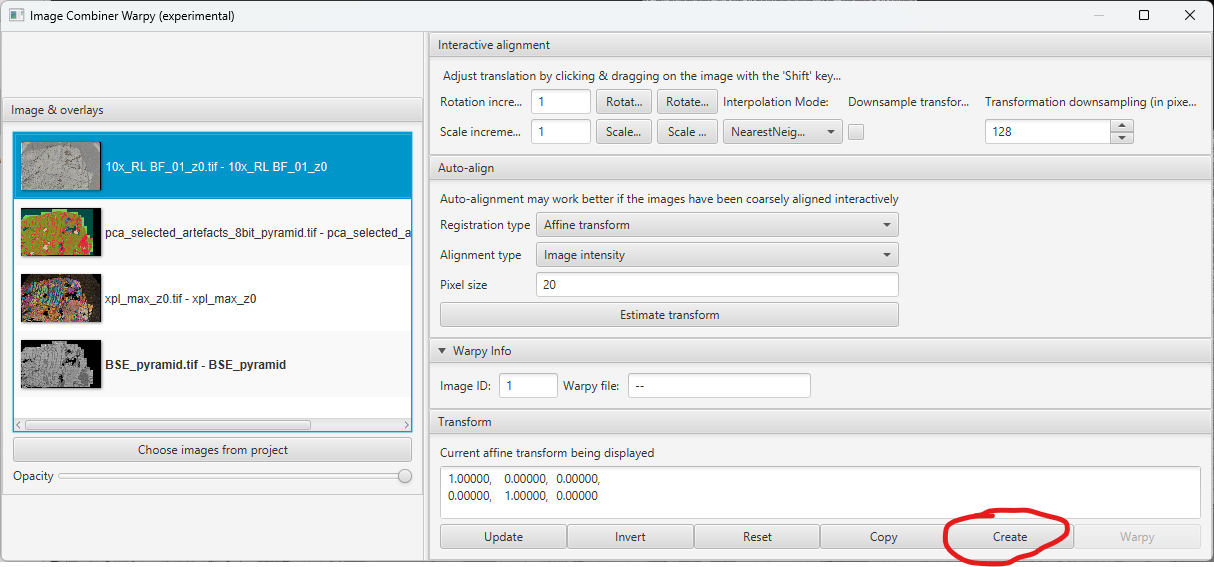
\includegraphics[width=5.75098in,height=2.68625in,alt={A screenshot of a computer AI-generated content may be incorrect.}]{./media/image19.png}
	
	\begin{enumerate}
		\def\labelenumi{\arabic{enumi}.}
		\setcounter{enumi}{4}
		\item
		A multi-channel image will be added in the data tree and opened*.
	\end{enumerate}
	
	*In old versions, you needed to: Go to the Annotation toolbar \textgreater{} Brightness \& contrast tool \textgreater{} tick on all (or custom selection). Then, click Create.
	
	\begin{enumerate}
		\def\labelenumi{\arabic{enumi}.}
		\setcounter{enumi}{5}
		\item
		Close ``Image Combiner Warpy (experimental)'' window.
	\end{enumerate}
	
	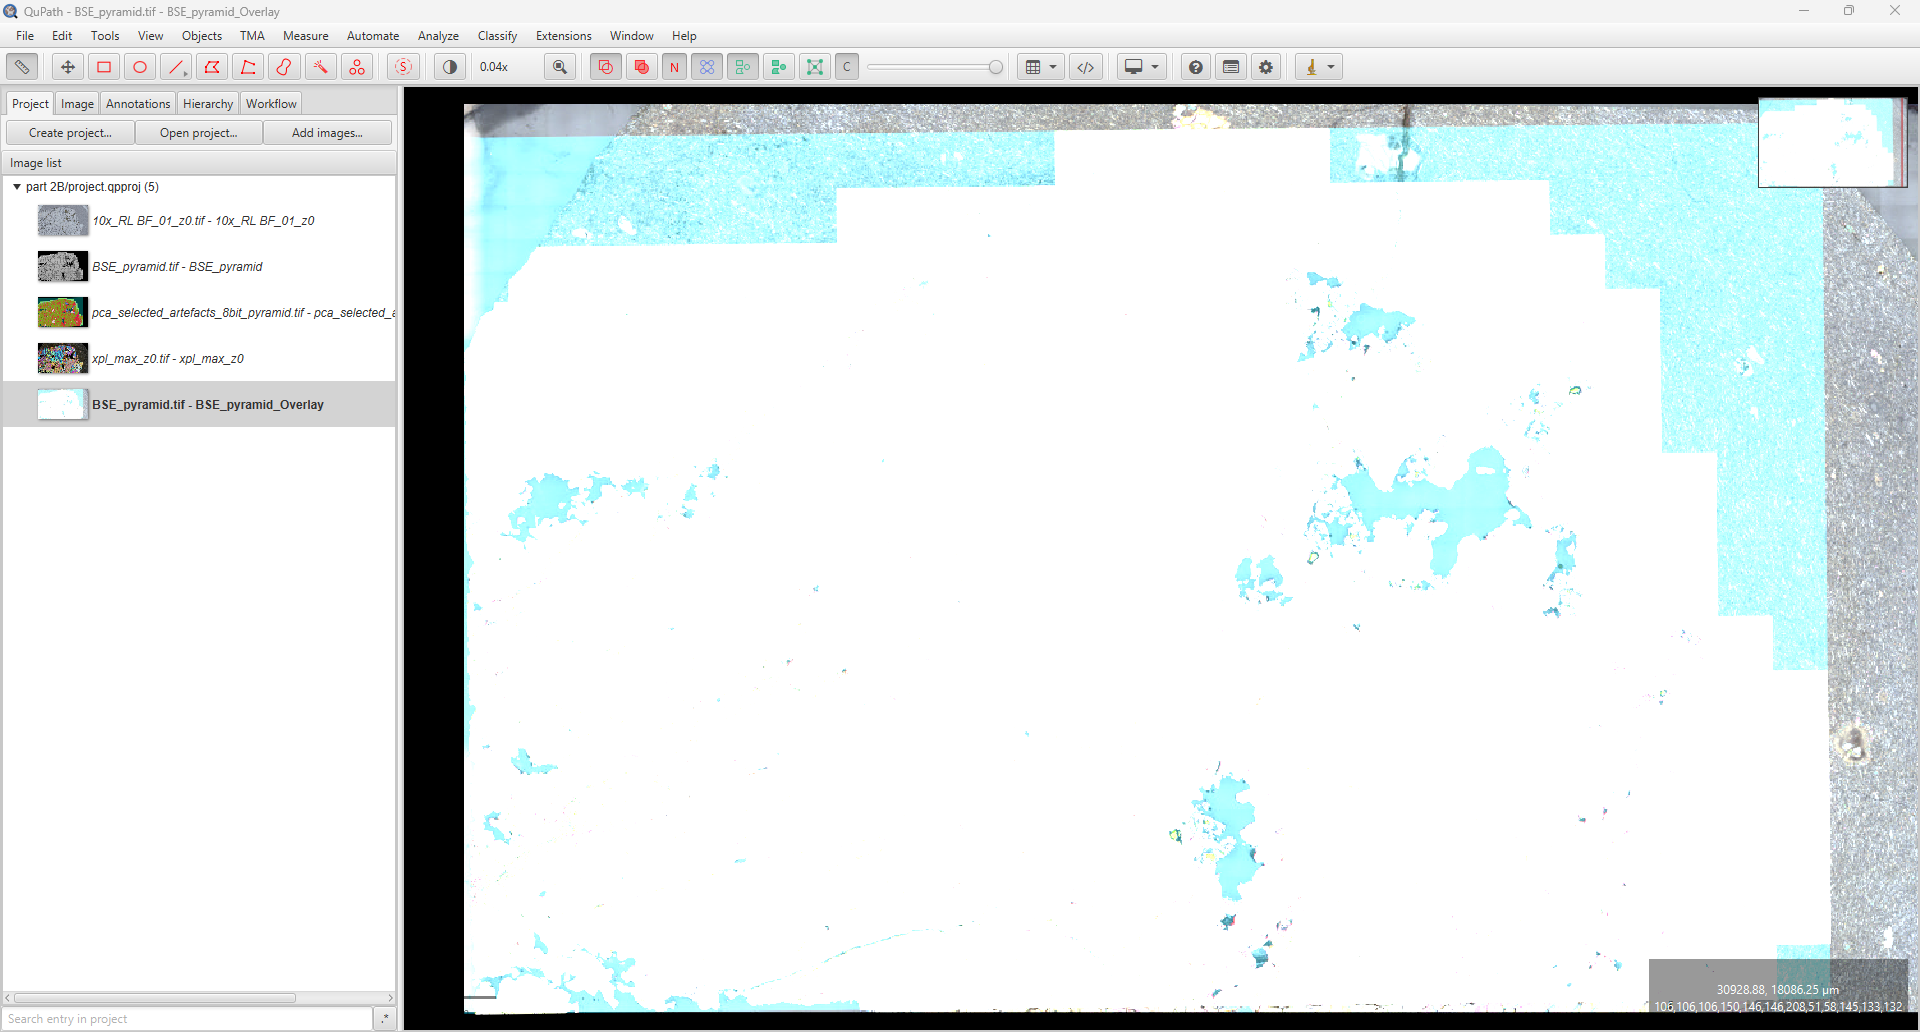
\includegraphics[width=6.26806in,height=3.36875in]{./media/image20.png}
	
	\begin{enumerate}
		\def\labelenumi{\arabic{enumi}.}
		\setcounter{enumi}{6}
		\item
		Optional: Compare the new image with the inputs. The multi-channel image has 12 channels (4 x 3-channels) as below:
	\end{enumerate}
	
	{\def\LTcaptype{none} % do not increment counter
		\begin{longtable}[]{@{}
				>{\raggedright\arraybackslash}p{(\linewidth - 2\tabcolsep) * \real{0.2711}}
				>{\raggedright\arraybackslash}p{(\linewidth - 2\tabcolsep) * \real{0.3429}}@{}}
			\toprule\noalign{}
			\begin{minipage}[b]{\linewidth}\raggedright
				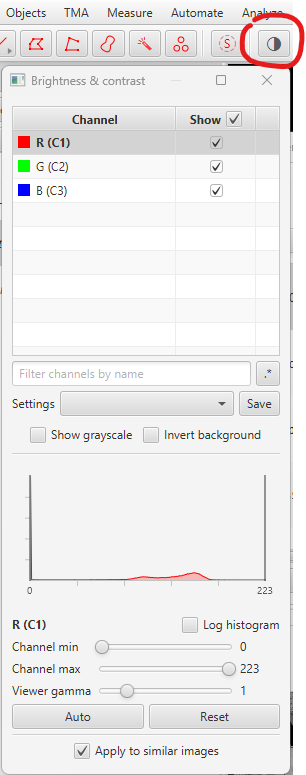
\includegraphics[width=1.54216in,height=3.90581in,alt={A screenshot of a computer AI-generated content may be incorrect.}]{./media/image21.png}
			\end{minipage} & \begin{minipage}[b]{\linewidth}\raggedright
				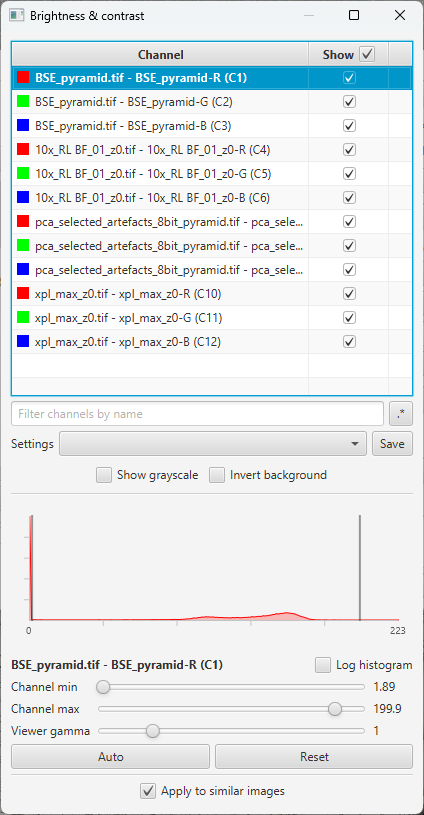
\includegraphics[width=1.99429in,height=3.83336in]{./media/image22.png}
			\end{minipage} \\
			\midrule\noalign{}
			\endhead
			\bottomrule\noalign{}
			\endlastfoot
		\end{longtable}
	}
	
	*You can improve the overlay appearance by deactivating all channels and only keeping red, green, and blue (RGB) of one source, corresponding to C1, C2, and C3 above.
	
	\paragraph{IV. Transfer annotations}\label{iv.-transfer-annotations}
	
	In your QuPath project, follow these steps:
	
	\begin{enumerate}
		\def\labelenumi{\arabic{enumi}.}
		\item
		Open the image(s) where the annotations were saved.
		\item
		Go to File \textgreater{} Export objects as GeoJSON\ldots{} \textgreater{} All objects \textgreater{} Save. If you have annotations in multiple images, repeat.
	\end{enumerate}
	
	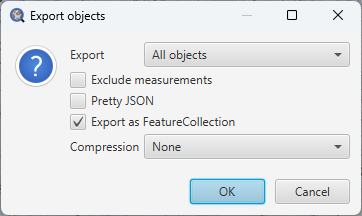
\includegraphics[width=3.77136in,height=2.25031in]{./media/image23.png}
	
	Pop up window:
	
	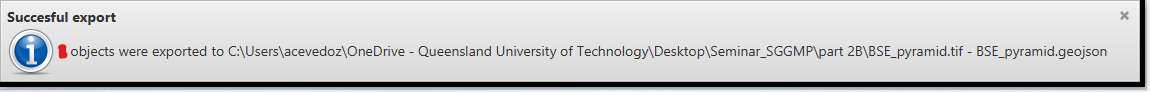
\includegraphics[width=6.26806in,height=0.50139in]{./media/image24.png}
	
	\begin{enumerate}
		\def\labelenumi{\arabic{enumi}.}
		\setcounter{enumi}{2}
		\item
		Open the multi-channel overlay.
		\item
		File \textgreater{} Import objects from file\ldots{}
		\item
		Find the QuPath project directory \textgreater{} select/Open ``*.geojson'' file. If you have annotations in multiple images, repeat.
		\item
		All annotations will now show in the overlay.
	\end{enumerate}
	
	\paragraph{V. Train and predict using a learning model}\label{v.-train-and-predict-using-a-learning-model}
	
	In your QuPath project, follow these steps:
	
	\begin{enumerate}
		\def\labelenumi{\arabic{enumi}.}
		\item
		Go to Menu toolbar \textgreater{} Classify \textgreater{} Pixel classification \textgreater{} Train pixel classifier...
		\item
		Select:
		
		\begin{enumerate}
			\def\labelenumii{\alph{enumii}.}
			\item
			Classifier \textgreater{} Random trees
			\item
			Resolution \textgreater{} Moderate (default)
		\end{enumerate}
	\end{enumerate}
	
	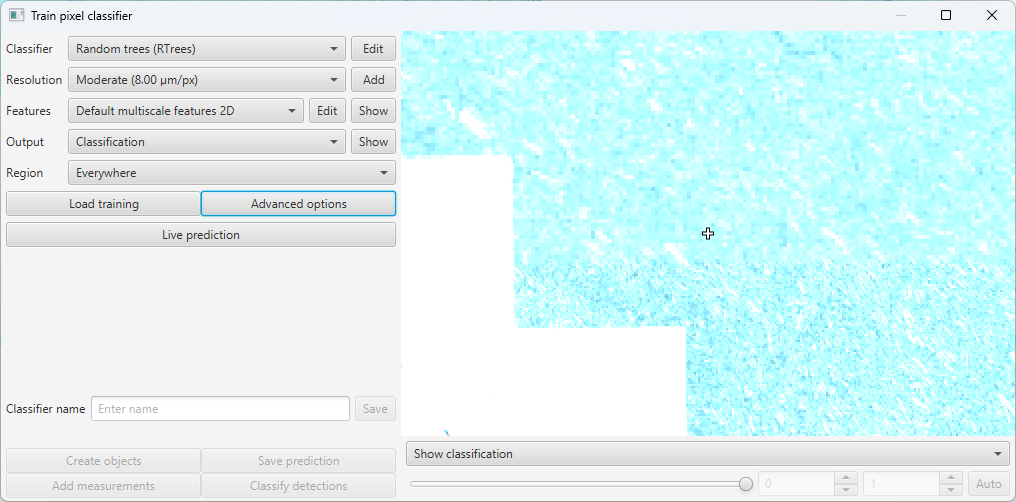
\includegraphics[width=6.26806in,height=3.09722in,alt={A screenshot of a computer AI-generated content may be incorrect.}]{./media/image25.png}
	
	\begin{enumerate}
		\def\labelenumi{\arabic{enumi}.}
		\setcounter{enumi}{2}
		\item
		Optional: Click Advanced options \textgreater{} Reweight samples (tick on)
	\end{enumerate}
	
	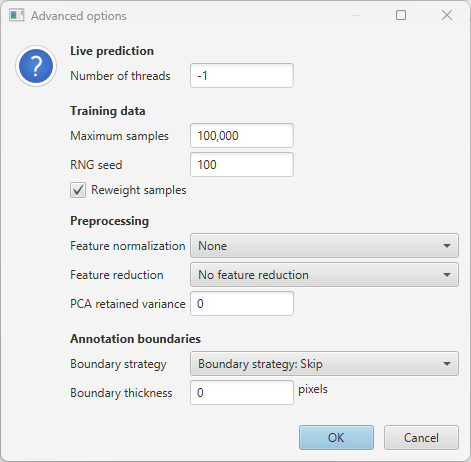
\includegraphics[width=2.92554in,height=2.86963in,alt={A screenshot of a computer AI-generated content may be incorrect.}]{./media/image26.png}
	
	\begin{enumerate}
		\def\labelenumi{\arabic{enumi}.}
		\setcounter{enumi}{3}
		\item
		Click Live prediction. Be patient, the interface will freeze for a few seconds.
		\item
		The slider at the top allows you to control the transparency of the segmented map for quality control.
	\end{enumerate}
	
	
\includegraphics[width=6.26806in,height=0.27361in]{./media/image27.png}
	
	\begin{enumerate}
		\def\labelenumi{\arabic{enumi}.}
		\setcounter{enumi}{5}
		\item
		Since you are in Live mode, you can draw more annotations (see ``II. Annotations''), right-click, and assign mineral class.
		
		\begin{enumerate}
			\def\labelenumii{\alph{enumii}.}
			\item
			This will improve your map but freeze the interface* to allow the model re-train with the new pixels.
			\item
			If you do not like freezing, try deactivating Live prediction, annotating more grains (that you remember), and activating Live when you are done.
		\end{enumerate}
		\item
		When satisfied, add a name for your classifier (``my\_first\_RT\_model'') and save (red circle below).
		\item
		Click ``Save prediction'' (blue circle below)
		\item
		Find the QuPath project directory \textgreater{} Save ``my\_first\_RT\_model.ome.tif'' file.
	\end{enumerate}
	
	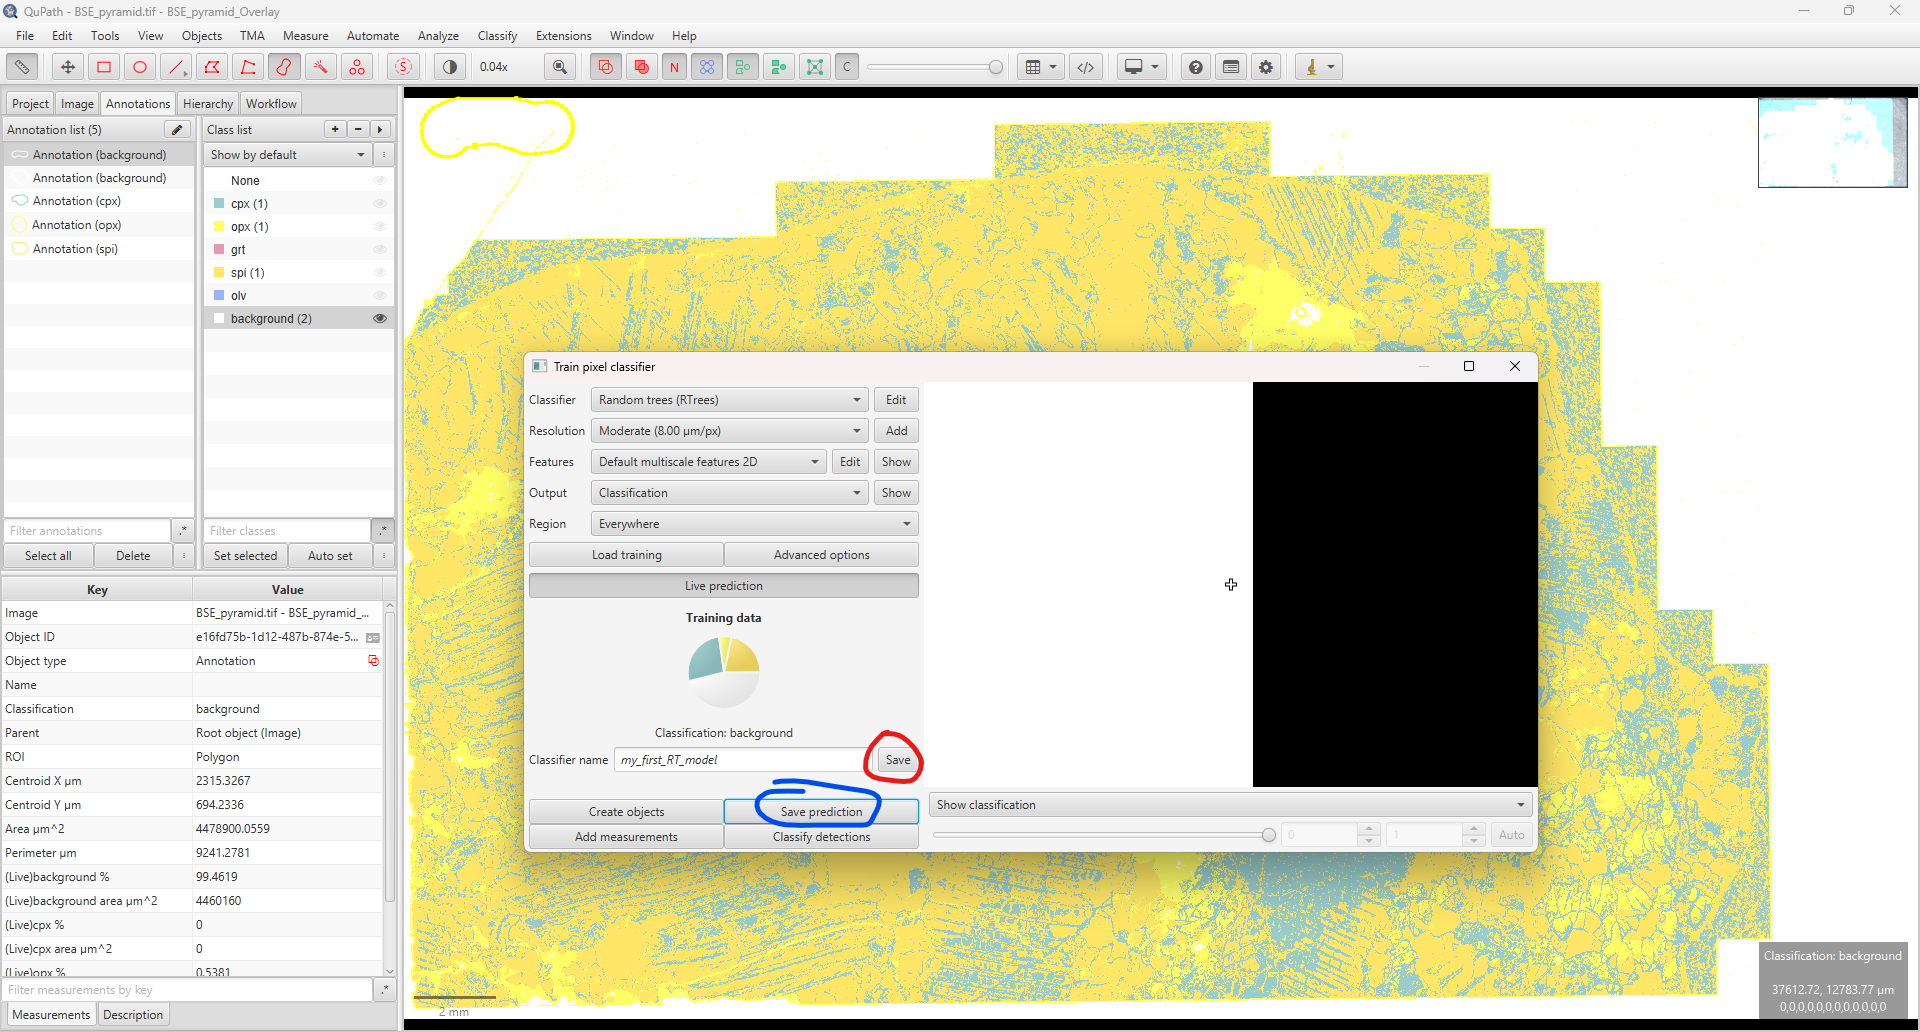
\includegraphics[width=6.26806in,height=3.36875in,alt={A screenshot of a computer AI-generated content may be incorrect.}]{./media/image28.png}
	
	In summary, `Live' segmentation tool has allowed you to rapidly classify pixels and learn more about your samples (beyond your annotation dataset). The technology highlights aspects in the whole-sample that were not sufficiently obvious for human vision and/or might have taken a very long to recognise and classify.
	
	Take home messages:
	
	\begin{itemize}
		\item
		This is an iterative process that uses hybrid-learning knowledge, colour, and texture.
		\item
		Since we are not using \ul{resource-intensive} spectral library search (as in the SEM), we have more control over the output.
		\item
		With practice, you will focus on \href{https://qupath.readthedocs.io/en/stable/docs/tutorials/pixel_classification.html}{features} that are resolvable and know when to change the settings, use less channels, or stop annotating.
		\item
		With data acquisition and processing \ul{consistency}, the trained model can be set up to predict new samples thanks to QuPath advanced scripting functionalities (\href{https://qupath.readthedocs.io/en/stable/docs/advanced/command_line.html\#passing-arguments-to-scripts}{without interface}).
	\end{itemize}
	
	\subsection{Part 3}\label{part-3}
	
	This part runs on Windows 11 and is given as extra learning material.
	
	\subsubsection{Exercise 1: Phase interpretation}\label{exercise-1-phase-interpretation}
	
	A user has segmented a sample for several purposes such as mineralogy (see Part 2B), texture (fractures, mineral zonation, etc.), or crystal orientation (using XPL-max index). The phase interpreter software was designed to read the predicted map (from the QuPath project directory) and output a custom mineral map where you can document and quantify the classified classes. It features:
	
	\begin{itemize}
		\item
		Editing of phase names into more accurate mineral/class (for publication)
		\item
		Basic sample display, area selection, and processing
		\item
		Image analysis for statistics (modal mineralogy, grain size distribution, association, accessibility) and measurements
		\item
		Saving partial analysis outputs into ``trial'' folders
	\end{itemize}
	
	The requirements are:
	
	\begin{itemize}
		\item
		You have not modified the names of your map or classifier. They need to match.
		\item
		The map can be loaded in memory (future work will implement pyramids).
	\end{itemize}
	
	On your Windows PC, follow these steps:
	
	\begin{enumerate}
		\def\labelenumi{\arabic{enumi}.}
		\item
		Open Phase interpreter
		\item
		(1) Define map
		
		\begin{enumerate}
			\def\labelenumii{\alph{enumii}.}
			\item
			QuPath project \textgreater{} "../Seminar\_material/exercises\_data/\textless your-project-folder\textgreater"
			\item
			Trained classifier \textgreater{} ``\textless name-of-your-classifier\textgreater''
			\item
			Background class \textgreater{} ``\textless name-of-background-classes\textgreater'' (e.g., glass, background, holes, marker pen). List classes that should not appear in the output) separated by a \ul{comma}.
			\item
			Click ``Generate preview''
		\end{enumerate}
		\item
		(2) Customise phase map
		
		\begin{enumerate}
			\def\labelenumii{\alph{enumii}.}
			\item
			Originals (ranked) \textgreater{} List of contained phases (equal to QuPath annotation names)
			\item
			Custom names \textgreater{} List where you can edit phases as minerals
			\item
			Targets \textgreater{} List where you can select the minerals to be shown (foreground)
			\item
			Region of interest (ROI) \textgreater{} click ``Draw'' for defining a ROI. It lowers the computational cost.
		\end{enumerate}
		\item
		(3) Choose the analysis
		
		\begin{enumerate}
			\def\labelenumii{\alph{enumii}.}
			\item
			Trial tag \textgreater{} ``\textless name-of-your-trial/ROI\textgreater''
			\item
			Generate \textgreater{} CTRL + click for selecting all (multiple analysis to be run)
			
			\begin{enumerate}
				\def\labelenumiii{\roman{enumiii}.}
				\item
				Association index matrix requires a search radius and connectivity (`four' recommended).
				\item
				Grain size distribution requires defining ``Pixel calibration''.
			\end{enumerate}
			\item
			Click ``Run''
		\end{enumerate}
	\end{enumerate}
	
	You were successful if your input looks like this (not for the websterite sample):
	
	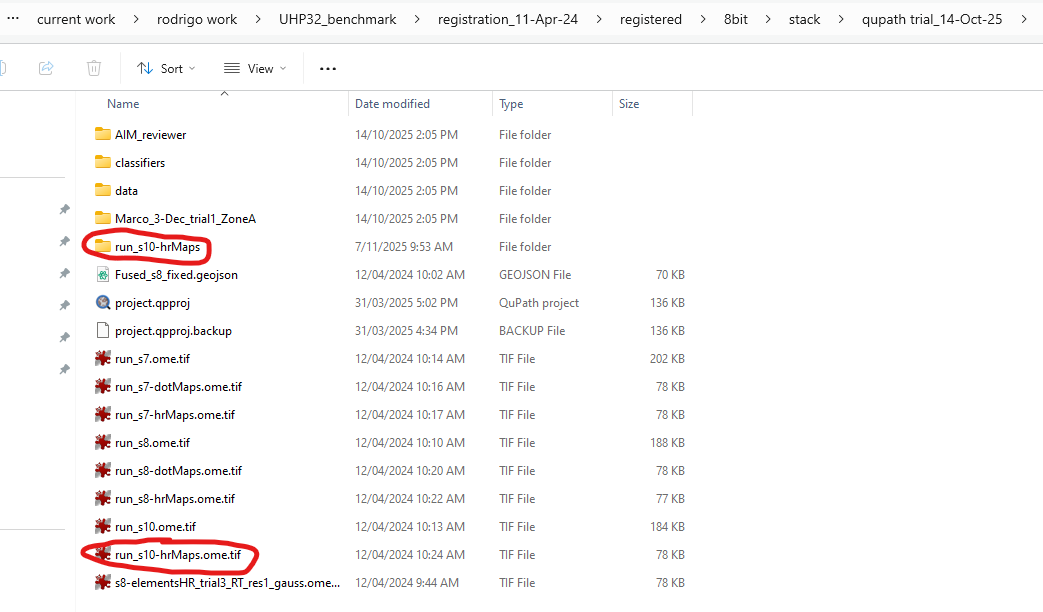
\includegraphics[width=5.20492in,height=3.05399in]{./media/image29.png}
	
	, and your output like this:
	
	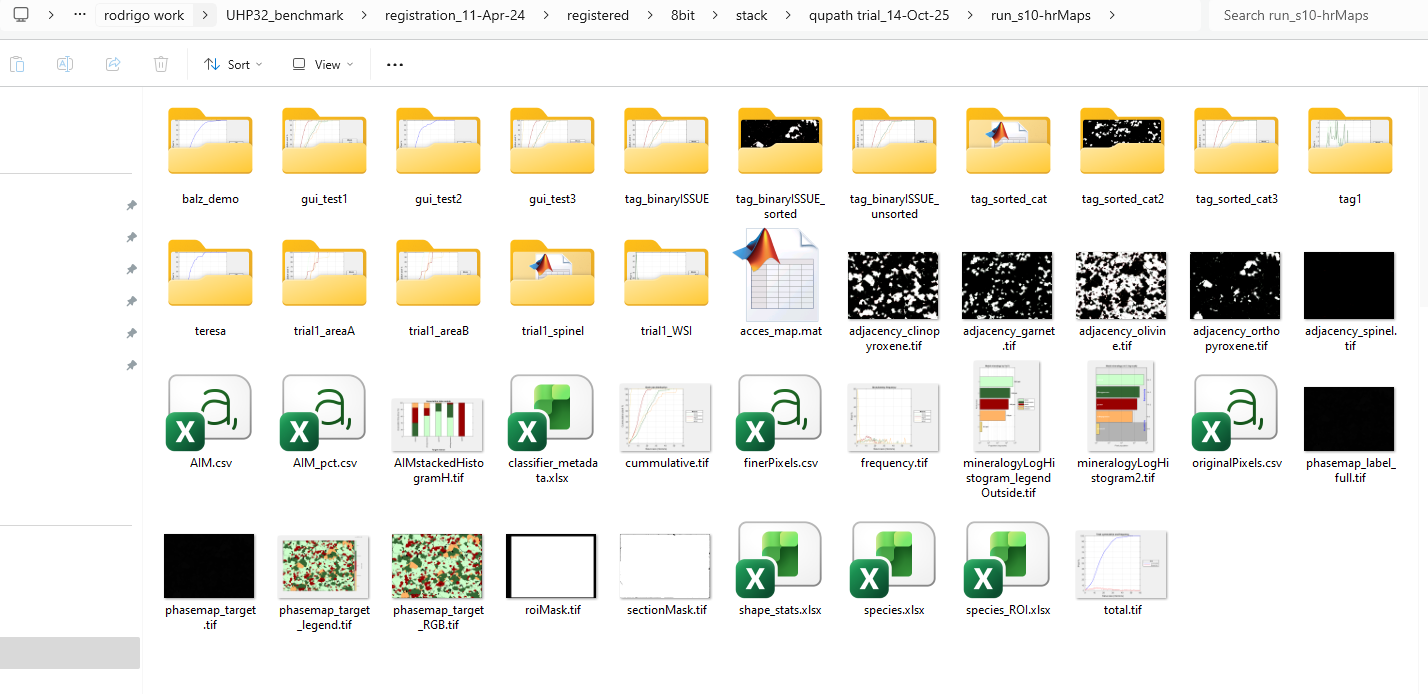
\includegraphics[width=6.26806in,height=3.04653in,alt={A screenshot of a computer AI-generated content may be incorrect.}]{./media/image30.png}
	
	, with several folders for each trial tag that was run.
	
	Finally, custom map outputs have applications such as doing new experiments on the interesting sample areas using new experiments and instruments that can ``jump'' between objects to acquire better spectra. There should be no need for brute force mapping (and saving) of all pixels if you can correlate techniques, e.g., `dot mapping' (Hrstka et al., 2018).
	
	\subsection{\texorpdfstring{Benchmark: }{Benchmark: }}\label{benchmark}
	
	\textbf{Garnet-websterite phase map.} After Scanning electron microscopy -- Backscattered electron and Energy dispersive spectroscopy (SEM-BSE/EDX) using default settings and spectral library search:
	
	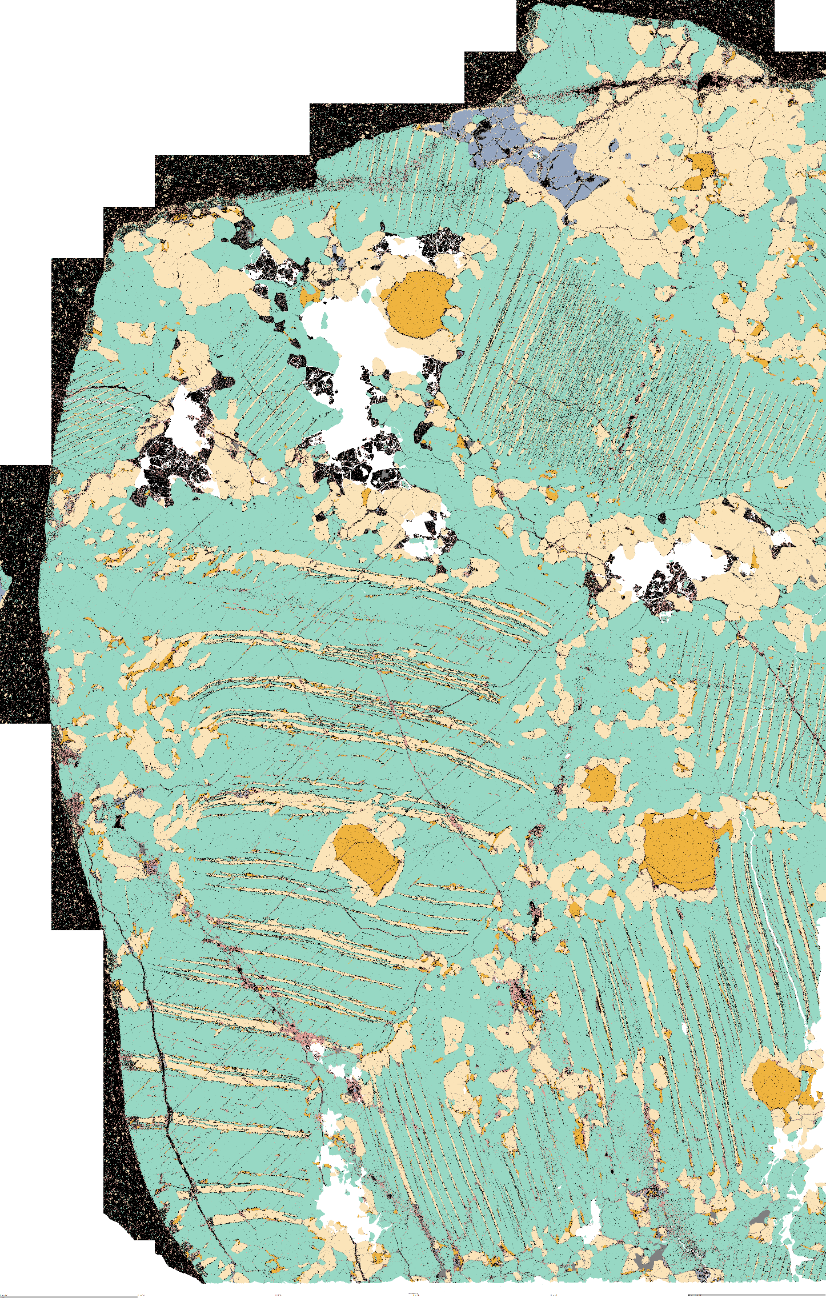
\includegraphics[width=5.34328in,height=8.38938in]{./media/image31.png}
	
	\textbf{Colour legend}
	
	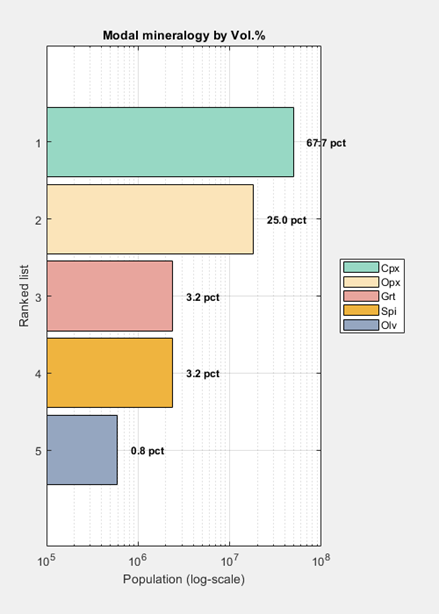
\includegraphics[width=2.92708in,height=4.09375in]{./media/image32.png} 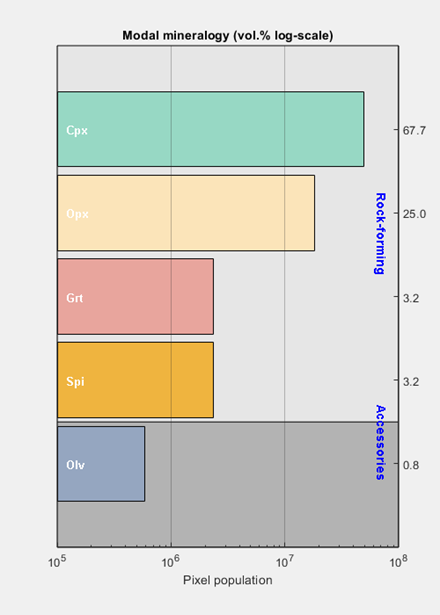
\includegraphics[width=2.93333in,height=4.10069in]{./media/image33.png}